\documentclass[twoside]{book}

% Packages required by doxygen
\usepackage{fixltx2e}
\usepackage{calc}
\usepackage{doxygen}
\usepackage[export]{adjustbox} % also loads graphicx
\usepackage{graphicx}
\usepackage[utf8]{inputenc}
\usepackage{makeidx}
\usepackage{multicol}
\usepackage{multirow}
\PassOptionsToPackage{warn}{textcomp}
\usepackage{textcomp}
\usepackage[nointegrals]{wasysym}
\usepackage[table]{xcolor}

% Font selection
\usepackage[T1]{fontenc}
\usepackage[scaled=.90]{helvet}
\usepackage{courier}
\usepackage{amssymb}
\usepackage{sectsty}
\renewcommand{\familydefault}{\sfdefault}
\allsectionsfont{%
  \fontseries{bc}\selectfont%
  \color{darkgray}%
}
\renewcommand{\DoxyLabelFont}{%
  \fontseries{bc}\selectfont%
  \color{darkgray}%
}
\newcommand{\+}{\discretionary{\mbox{\scriptsize$\hookleftarrow$}}{}{}}

% Page & text layout
\usepackage{geometry}
\geometry{%
  a4paper,%
  top=2.5cm,%
  bottom=2.5cm,%
  left=2.5cm,%
  right=2.5cm%
}
\tolerance=750
\hfuzz=15pt
\hbadness=750
\setlength{\emergencystretch}{15pt}
\setlength{\parindent}{0cm}
\setlength{\parskip}{0.2cm}
\makeatletter
\renewcommand{\paragraph}{%
  \@startsection{paragraph}{4}{0ex}{-1.0ex}{1.0ex}{%
    \normalfont\normalsize\bfseries\SS@parafont%
  }%
}
\renewcommand{\subparagraph}{%
  \@startsection{subparagraph}{5}{0ex}{-1.0ex}{1.0ex}{%
    \normalfont\normalsize\bfseries\SS@subparafont%
  }%
}
\makeatother

% Headers & footers
\usepackage{fancyhdr}
\pagestyle{fancyplain}
\fancyhead[LE]{\fancyplain{}{\bfseries\thepage}}
\fancyhead[CE]{\fancyplain{}{}}
\fancyhead[RE]{\fancyplain{}{\bfseries\leftmark}}
\fancyhead[LO]{\fancyplain{}{\bfseries\rightmark}}
\fancyhead[CO]{\fancyplain{}{}}
\fancyhead[RO]{\fancyplain{}{\bfseries\thepage}}
\fancyfoot[LE]{\fancyplain{}{}}
\fancyfoot[CE]{\fancyplain{}{}}
\fancyfoot[RE]{\fancyplain{}{\bfseries\scriptsize Generated by Doxygen }}
\fancyfoot[LO]{\fancyplain{}{\bfseries\scriptsize Generated by Doxygen }}
\fancyfoot[CO]{\fancyplain{}{}}
\fancyfoot[RO]{\fancyplain{}{}}
\renewcommand{\footrulewidth}{0.4pt}
\renewcommand{\chaptermark}[1]{%
  \markboth{#1}{}%
}
\renewcommand{\sectionmark}[1]{%
  \markright{\thesection\ #1}%
}

% Indices & bibliography
\usepackage{natbib}
\usepackage[titles]{tocloft}
\setcounter{tocdepth}{3}
\setcounter{secnumdepth}{5}
\makeindex

% Hyperlinks (required, but should be loaded last)
\usepackage{ifpdf}
\ifpdf
  \usepackage[pdftex,pagebackref=true]{hyperref}
\else
  \usepackage[ps2pdf,pagebackref=true]{hyperref}
\fi
\hypersetup{%
  colorlinks=true,%
  linkcolor=blue,%
  citecolor=blue,%
  unicode%
}

% Custom commands
\newcommand{\clearemptydoublepage}{%
  \newpage{\pagestyle{empty}\cleardoublepage}%
}


%===== C O N T E N T S =====

\begin{document}

% Titlepage & ToC
\hypersetup{pageanchor=false,
             bookmarks=true,
             bookmarksnumbered=true,
             pdfencoding=unicode
            }
\pagenumbering{roman}
\begin{titlepage}
\vspace*{7cm}
\begin{center}%
{\Large Glex }\\
\vspace*{1cm}
{\large Generated by Doxygen 1.8.10}\\
\end{center}
\end{titlepage}
\clearemptydoublepage
\tableofcontents
\clearemptydoublepage
\pagenumbering{arabic}
\hypersetup{pageanchor=true}

%--- Begin generated contents ---
\chapter{Prerequisites}
\label{md_README}
\hypertarget{md_README}{}

\begin{DoxyItemize}
\item G\+N\+U Autotools
\item Open\+G\+L 3.\+0
\item C++11 compiler (tested with G\+C\+C 4.\+8.\+3+)
\item \href{http://www.boost.org/}{\tt Boost}
\item \href{http://glew.sourceforge.net/}{\tt G\+L\+E\+W}
\item \href{https://www.libsdl.org/}{\tt S\+D\+L2}
\item \href{http://glm.g-truc.net/}{\tt G\+L\+M}
\end{DoxyItemize}

On Fedora 20 or later you can install these using a single command (as root)\+:

\begin{quote}
\$ yum install boost-\/$\ast$ glew-\/devel S\+D\+L2\+\_\+$\ast$ glm-\/devel \end{quote}


\section*{Building}

After cloning the source code or extracting a distributed archive, change to the directory where the source code is\+:


\begin{DoxyCode}
1 $ autoreconf -i
2 $ ./configure
3 $ make
\end{DoxyCode}


Alternatively, if you\textquotesingle{}d like to build the project in debug mode use\+:

\begin{quote}
\$ make C\+X\+X\+F\+L\+A\+G\+S=-\/\+D\+D\+E\+B\+U\+G \end{quote}


\section*{Running}

The build process should create a binary that can be executed as follows\+:

\begin{quote}
\$ ./src/shaderexample \end{quote}


See

\begin{quote}
\$ ./src/shaderexample --help \end{quote}


for usage instructions. 
\chapter{Hierarchical Index}
\section{Class Hierarchy}
This inheritance list is sorted roughly, but not completely, alphabetically\+:\begin{DoxyCompactList}
\item \contentsline{section}{Bounding\+Box}{\pageref{class_bounding_box}}{}
\item \contentsline{section}{Camera}{\pageref{class_camera}}{}
\item \contentsline{section}{Game}{\pageref{class_game}}{}
\item \contentsline{section}{Game\+Asset}{\pageref{class_game_asset}}{}
\begin{DoxyCompactList}
\item \contentsline{section}{Cube\+Asset}{\pageref{class_cube_asset}}{}
\item \contentsline{section}{Floor\+Asset}{\pageref{class_floor_asset}}{}
\item \contentsline{section}{Pyramid\+Asset}{\pageref{class_pyramid_asset}}{}
\end{DoxyCompactList}
\item \contentsline{section}{Game\+Asset\+Manager}{\pageref{class_game_asset_manager}}{}
\item \contentsline{section}{Game\+World}{\pageref{class_game_world}}{}
\item \contentsline{section}{Python\+B}{\pageref{class_python_b}}{}
\item \contentsline{section}{S\+D\+L\+Window\+Deleter}{\pageref{struct_s_d_l_window_deleter}}{}
\end{DoxyCompactList}

\chapter{Class Index}
\section{Class List}
Here are the classes, structs, unions and interfaces with brief descriptions\+:\begin{DoxyCompactList}
\item\contentsline{section}{\hyperlink{classCubeAsset}{Cube\+Asset} }{\pageref{classCubeAsset}}{}
\item\contentsline{section}{\hyperlink{classFloorAsset}{Floor\+Asset} }{\pageref{classFloorAsset}}{}
\item\contentsline{section}{\hyperlink{classGameAsset}{Game\+Asset} }{\pageref{classGameAsset}}{}
\item\contentsline{section}{\hyperlink{classGameAssetManager}{Game\+Asset\+Manager} \\*\hyperlink{classGameAssetManager}{Game\+Asset\+Manager} is a container for Game\+Assets }{\pageref{classGameAssetManager}}{}
\item\contentsline{section}{\hyperlink{classGameWorld}{Game\+World} \\*\hyperlink{classGameWorld}{Game\+World} allows us to separate the management of the game world from the nuts and bolts of game loop initialisation }{\pageref{classGameWorld}}{}
\item\contentsline{section}{\hyperlink{classPyramidAsset}{Pyramid\+Asset} }{\pageref{classPyramidAsset}}{}
\item\contentsline{section}{\hyperlink{structSDLWindowDeleter}{S\+D\+L\+Window\+Deleter} }{\pageref{structSDLWindowDeleter}}{}
\end{DoxyCompactList}

\chapter{File Index}
\section{File List}
Here is a list of all files with brief descriptions\+:\begin{DoxyCompactList}
\item\contentsline{section}{\hyperlink{config_8h}{config.\+h} }{\pageref{config_8h}}{}
\item\contentsline{section}{src/\hyperlink{common_8h}{common.\+h} }{\pageref{common_8h}}{}
\item\contentsline{section}{src/\hyperlink{CubeAsset_8cc}{Cube\+Asset.\+cc} }{\pageref{CubeAsset_8cc}}{}
\item\contentsline{section}{src/\hyperlink{CubeAsset_8h}{Cube\+Asset.\+h} }{\pageref{CubeAsset_8h}}{}
\item\contentsline{section}{src/\hyperlink{FloorAsset_8cc}{Floor\+Asset.\+cc} }{\pageref{FloorAsset_8cc}}{}
\item\contentsline{section}{src/\hyperlink{FloorAsset_8h}{Floor\+Asset.\+h} }{\pageref{FloorAsset_8h}}{}
\item\contentsline{section}{src/\hyperlink{GameAsset_8h}{Game\+Asset.\+h} }{\pageref{GameAsset_8h}}{}
\item\contentsline{section}{src/\hyperlink{GameAssetManager_8cc}{Game\+Asset\+Manager.\+cc} }{\pageref{GameAssetManager_8cc}}{}
\item\contentsline{section}{src/\hyperlink{GameAssetManager_8h}{Game\+Asset\+Manager.\+h} }{\pageref{GameAssetManager_8h}}{}
\item\contentsline{section}{src/\hyperlink{GameWorld_8cc}{Game\+World.\+cc} }{\pageref{GameWorld_8cc}}{}
\item\contentsline{section}{src/\hyperlink{GameWorld_8h}{Game\+World.\+h} }{\pageref{GameWorld_8h}}{}
\item\contentsline{section}{src/\hyperlink{main_8cc}{main.\+cc} }{\pageref{main_8cc}}{}
\item\contentsline{section}{src/\hyperlink{PyramidAsset_8cc}{Pyramid\+Asset.\+cc} }{\pageref{PyramidAsset_8cc}}{}
\item\contentsline{section}{src/\hyperlink{PyramidAsset_8h}{Pyramid\+Asset.\+h} }{\pageref{PyramidAsset_8h}}{}
\end{DoxyCompactList}

\chapter{Class Documentation}
\hypertarget{classCubeAsset}{}\section{Cube\+Asset Class Reference}
\label{classCubeAsset}\index{Cube\+Asset@{Cube\+Asset}}


{\ttfamily \#include $<$Cube\+Asset.\+h$>$}



Inheritance diagram for Cube\+Asset\+:
\nopagebreak
\begin{figure}[H]
\begin{center}
\leavevmode
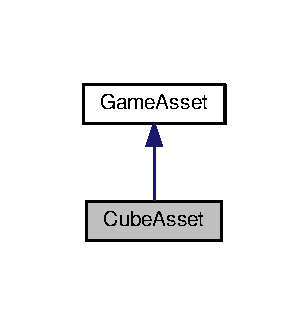
\includegraphics[width=148pt]{classCubeAsset__inherit__graph}
\end{center}
\end{figure}


Collaboration diagram for Cube\+Asset\+:
\nopagebreak
\begin{figure}[H]
\begin{center}
\leavevmode
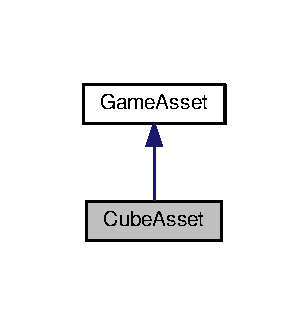
\includegraphics[width=148pt]{classCubeAsset__coll__graph}
\end{center}
\end{figure}
\subsection*{Public Member Functions}
\begin{DoxyCompactItemize}
\item 
\hyperlink{classCubeAsset_a0252e564114a3cda7e3911ef95742a34}{Cube\+Asset} (G\+Lfloat x, G\+Lfloat y, G\+Lfloat z)
\item 
\hyperlink{classCubeAsset_ab3ab9a5da82cbf8537a28652410093b1}{$\sim$\+Cube\+Asset} ()
\item 
virtual void \hyperlink{classCubeAsset_a1af568486056e254ffcf98fd99947bfe}{Draw} (G\+Luint)
\end{DoxyCompactItemize}
\subsection*{Private Member Functions}
\begin{DoxyCompactItemize}
\item 
void \hyperlink{classCubeAsset_ac3855728a8d6c1612ebc85f82d3b535e}{check\+Error} (std\+::string file, int line)
\end{DoxyCompactItemize}
\subsection*{Private Attributes}
\begin{DoxyCompactItemize}
\item 
G\+Luint \hyperlink{classCubeAsset_ac66c2ec869f392515dad4ebda1fe4792}{element\+\_\+buffer\+\_\+length}
\item 
G\+Luint \hyperlink{classCubeAsset_ac4c2395c395e9bcebc5d15d425a505ec}{color\+\_\+buffer\+\_\+length}
\item 
G\+Luint \hyperlink{classCubeAsset_a3054ed8a7d6cc1575aebdfc40038847b}{vertex\+\_\+buffer\+\_\+length}
\item 
G\+Luint \hyperlink{classCubeAsset_a31bd098f60e2c24988316a9cc9335987}{vertex\+\_\+buffer\+\_\+token}
\item 
G\+Luint \hyperlink{classCubeAsset_a4cb558d463a5fa01ba7fdd884e697a73}{color\+\_\+buffer\+\_\+token}
\item 
G\+Luint \hyperlink{classCubeAsset_a4fae699256e7c5633a8174a93ca8a0ec}{element\+\_\+buffer\+\_\+token}
\end{DoxyCompactItemize}


\subsection{Constructor \& Destructor Documentation}
\hypertarget{classCubeAsset_a0252e564114a3cda7e3911ef95742a34}{}\index{Cube\+Asset@{Cube\+Asset}!Cube\+Asset@{Cube\+Asset}}
\index{Cube\+Asset@{Cube\+Asset}!Cube\+Asset@{Cube\+Asset}}
\subsubsection[{Cube\+Asset(\+G\+Lfloat x, G\+Lfloat y, G\+Lfloat z)}]{\setlength{\rightskip}{0pt plus 5cm}Cube\+Asset\+::\+Cube\+Asset (
\begin{DoxyParamCaption}
\item[{G\+Lfloat}]{x, }
\item[{G\+Lfloat}]{y, }
\item[{G\+Lfloat}]{z}
\end{DoxyParamCaption}
)}\label{classCubeAsset_a0252e564114a3cda7e3911ef95742a34}
Cube Creation models coordinates, origin dependant on xyz variables. vertex buffer models coordinates, for the triangles. colour buffer models the colour of the object triangles. element buffer creates the cube using 12 triangles.

Buffer Implementation Transfer buffers to the G\+P\+U
\begin{DoxyCode}
3                                                     \{
4 
12 
13   GLfloat vertex\_buffer [] \{
14       -0.5f + x, -0.5f + y, -0.5f + z   \textcolor{comment}{//0}
15     , -0.5f + x,  0.5f + y, -0.5f + z   \textcolor{comment}{//1}
16     ,  0.5f + x, -0.5f + y, -0.5f + z   \textcolor{comment}{//2}
17     ,  0.5f + x,  0.5f + y, -0.5f + z   \textcolor{comment}{//3}
18     , -0.5f + x, -0.5f + y,  0.5f + z   \textcolor{comment}{//5}
19     , -0.5f + x,  0.5f + y,  0.5f + z   \textcolor{comment}{//4}
20     ,  0.5f + x, -0.5f + y,  0.5f + z   \textcolor{comment}{//6}
21     ,  0.5f + x,  0.5f + y,  0.5f + z   \textcolor{comment}{//7}
22   \};
23   \hyperlink{classCubeAsset_a3054ed8a7d6cc1575aebdfc40038847b}{vertex\_buffer\_length} = \textcolor{keyword}{sizeof}(vertex\_buffer);
24 
25   GLfloat color\_buffer [] \{
26       1.000f, 1.000f, 0.000f \textcolor{comment}{//0}
27     , 1.000f, 1.000f, 0.000f \textcolor{comment}{//1}
28     , 1.000f, 1.000f, 0.000f \textcolor{comment}{//2}
29     , 1.000f, 1.000f, 0.000f \textcolor{comment}{//3}
30     , 1.000f, 1.000f, 0.000f \textcolor{comment}{//4}
31     , 1.000f, 1.000f, 0.000f \textcolor{comment}{//5}
32     , 1.000f, 1.000f, 0.000f \textcolor{comment}{//6}
33     , 1.000f, 1.000f, 0.000f \textcolor{comment}{//7}
34   \};
35   \hyperlink{classCubeAsset_ac4c2395c395e9bcebc5d15d425a505ec}{color\_buffer\_length} = \textcolor{keyword}{sizeof}(color\_buffer);
36 
37   GLuint element\_buffer []  \{
38       0, 1, 2  \textcolor{comment}{// front}
39     , 1, 3, 2  
40     , 4, 5, 6  \textcolor{comment}{// back}
41     , 5, 7, 6  
42     , 1, 5, 3  \textcolor{comment}{// top}
43     , 5, 7, 3 
44     , 0, 1, 4  \textcolor{comment}{// left}
45     , 1, 5, 4  
46     , 2, 3, 6  \textcolor{comment}{// right}
47     , 3, 7, 6  
48     , 0, 4, 2  \textcolor{comment}{// bottom}
49     , 4, 2, 6     
50   \};
51   \hyperlink{classCubeAsset_ac66c2ec869f392515dad4ebda1fe4792}{element\_buffer\_length} = \textcolor{keyword}{sizeof}(element\_buffer);
52 
57 
58   \textcolor{comment}{// create vertex buffer}
59   glGenBuffers(1, &\hyperlink{classCubeAsset_a31bd098f60e2c24988316a9cc9335987}{vertex\_buffer\_token});
60   \textcolor{comment}{// immediately bind the buffer and transfer the data}
61   glBindBuffer(GL\_ARRAY\_BUFFER, \hyperlink{classCubeAsset_a31bd098f60e2c24988316a9cc9335987}{vertex\_buffer\_token});
62   glBufferData(GL\_ARRAY\_BUFFER, \hyperlink{classCubeAsset_a3054ed8a7d6cc1575aebdfc40038847b}{vertex\_buffer\_length}, vertex\_buffer, GL\_STATIC\_DRAW);
63 
64   \textcolor{comment}{// create color buffer}
65   glGenBuffers(1, &\hyperlink{classCubeAsset_a4cb558d463a5fa01ba7fdd884e697a73}{color\_buffer\_token});
66   \textcolor{comment}{// immediately bind the buffer and transfer the data}
67   glBindBuffer(GL\_ARRAY\_BUFFER, \hyperlink{classCubeAsset_a4cb558d463a5fa01ba7fdd884e697a73}{color\_buffer\_token});
68   glBufferData(GL\_ARRAY\_BUFFER, \hyperlink{classCubeAsset_ac4c2395c395e9bcebc5d15d425a505ec}{color\_buffer\_length}, color\_buffer, GL\_STATIC\_DRAW);
69   
70   glGenBuffers(1, &\hyperlink{classCubeAsset_a4fae699256e7c5633a8174a93ca8a0ec}{element\_buffer\_token});
71   glBindBuffer(GL\_ELEMENT\_ARRAY\_BUFFER, \hyperlink{classCubeAsset_a4fae699256e7c5633a8174a93ca8a0ec}{element\_buffer\_token});
72   glBufferData(GL\_ELEMENT\_ARRAY\_BUFFER, \hyperlink{classCubeAsset_ac66c2ec869f392515dad4ebda1fe4792}{element\_buffer\_length}, element\_buffer, 
      GL\_STATIC\_DRAW);
73 \}
\end{DoxyCode}
\hypertarget{classCubeAsset_ab3ab9a5da82cbf8537a28652410093b1}{}\index{Cube\+Asset@{Cube\+Asset}!````~Cube\+Asset@{$\sim$\+Cube\+Asset}}
\index{````~Cube\+Asset@{$\sim$\+Cube\+Asset}!Cube\+Asset@{Cube\+Asset}}
\subsubsection[{$\sim$\+Cube\+Asset()}]{\setlength{\rightskip}{0pt plus 5cm}Cube\+Asset\+::$\sim$\+Cube\+Asset (
\begin{DoxyParamCaption}
{}
\end{DoxyParamCaption}
)}\label{classCubeAsset_ab3ab9a5da82cbf8537a28652410093b1}

\begin{DoxyCode}
75                       \{
76 \}
\end{DoxyCode}


\subsection{Member Function Documentation}
\hypertarget{classCubeAsset_ac3855728a8d6c1612ebc85f82d3b535e}{}\index{Cube\+Asset@{Cube\+Asset}!check\+Error@{check\+Error}}
\index{check\+Error@{check\+Error}!Cube\+Asset@{Cube\+Asset}}
\subsubsection[{check\+Error(std\+::string file, int line)}]{\setlength{\rightskip}{0pt plus 5cm}void Cube\+Asset\+::check\+Error (
\begin{DoxyParamCaption}
\item[{std\+::string}]{file, }
\item[{int}]{line}
\end{DoxyParamCaption}
)\hspace{0.3cm}{\ttfamily [private]}}\label{classCubeAsset_ac3855728a8d6c1612ebc85f82d3b535e}

\begin{DoxyCode}
85                                                    \{
86   GLenum gl\_error = glGetError();
87   \textcolor{keywordflow}{if}(GL\_NO\_ERROR != gl\_error) \{
88     std::cerr << \textcolor{stringliteral}{"GL error in "} << file << \textcolor{stringliteral}{" at line "} << line << \textcolor{stringliteral}{" error: "} << gl\_error << std::endl;
89     exit(-1);
90   \}
91 \}
\end{DoxyCode}
\hypertarget{classCubeAsset_a1af568486056e254ffcf98fd99947bfe}{}\index{Cube\+Asset@{Cube\+Asset}!Draw@{Draw}}
\index{Draw@{Draw}!Cube\+Asset@{Cube\+Asset}}
\subsubsection[{Draw(\+G\+Luint)}]{\setlength{\rightskip}{0pt plus 5cm}void Cube\+Asset\+::\+Draw (
\begin{DoxyParamCaption}
\item[{G\+Luint}]{program\+\_\+token}
\end{DoxyParamCaption}
)\hspace{0.3cm}{\ttfamily [virtual]}}\label{classCubeAsset_a1af568486056e254ffcf98fd99947bfe}
Buffer Arrays use the previously transferred buffer as the vertex array. This way we transfer the buffer once -- at construction -- not on every frame.

Implements \hyperlink{classGameAsset_a961aa51ca0a9961fc584c0b5d5431300}{Game\+Asset}.


\begin{DoxyCode}
93                                          \{
94   \textcolor{keywordflow}{if}(!glIsProgram(program\_token)) \{
95     std::cerr << \textcolor{stringliteral}{"Drawing Cube with invalid program"} << std::endl;
96     \textcolor{keywordflow}{return};
97   \}
98   GLint validation\_ok;
99   glValidateProgram(program\_token);
100   glGetProgramiv(program\_token, GL\_VALIDATE\_STATUS, &validation\_ok);
101   \textcolor{keywordflow}{if}(!validation\_ok) \{
102     GLint maxLength = 0;
103     glGetProgramiv(program\_token, GL\_INFO\_LOG\_LENGTH, &maxLength);
104 
105     \textcolor{comment}{//The maxLength includes the NULL character}
106     std::vector<char> errorLog(maxLength);
107     glGetProgramInfoLog(program\_token, maxLength, &maxLength, &errorLog[0]);
108 
109     std::cerr << \textcolor{stringliteral}{"Invalid program "} << program\_token << \textcolor{stringliteral}{" with error code "} << validation\_ok << std::endl;
110     \textcolor{keywordflow}{for}(\textcolor{keyword}{auto} c: errorLog) \{
111       std::cerr << c;
112     \}
113     exit(-1);
114   \}
115 
116   GLuint position\_attrib = glGetAttribLocation(program\_token, \textcolor{stringliteral}{"position"});
117   \hyperlink{CubeAsset_8cc_a75f201b0e53e68726854997957322b8d}{checkGLError}();
118 
119   glUseProgram(program\_token);
120   \hyperlink{CubeAsset_8cc_a75f201b0e53e68726854997957322b8d}{checkGLError}();
121 
127   glEnableVertexAttribArray(0);
128 
129   glBindBuffer(GL\_ARRAY\_BUFFER, \hyperlink{classCubeAsset_a31bd098f60e2c24988316a9cc9335987}{vertex\_buffer\_token});
130   glVertexAttribPointer(
131                         position\_attrib,               \textcolor{comment}{/* attribute */}
132                         3,                             \textcolor{comment}{/* size */}
133                         GL\_FLOAT,                      \textcolor{comment}{/* type */}
134                         GL\_FALSE,                      \textcolor{comment}{/* normalized? */}
135                         0,                             \textcolor{comment}{/* stride */}
136                         (\textcolor{keywordtype}{void}*)0                       \textcolor{comment}{/* array buffer offset */}
137                         );
138   glEnableVertexAttribArray(position\_attrib);
139 
140   \hyperlink{CubeAsset_8cc_a75f201b0e53e68726854997957322b8d}{checkGLError}();
141 
142   glBindBuffer(GL\_ARRAY\_BUFFER, \hyperlink{classCubeAsset_a4cb558d463a5fa01ba7fdd884e697a73}{color\_buffer\_token});
143   glVertexAttribPointer(
144                         1,                             \textcolor{comment}{/* attribute */}
145                         3,                             \textcolor{comment}{/* size */}
146                         GL\_FLOAT,                      \textcolor{comment}{/* type */}
147                         GL\_FALSE,                      \textcolor{comment}{/* normalized? */}
148                         0,                             \textcolor{comment}{/* stride */}
149                         (\textcolor{keywordtype}{void}*)0                       \textcolor{comment}{/* array buffer offset */}
150                         );
151 
152   \hyperlink{CubeAsset_8cc_a75f201b0e53e68726854997957322b8d}{checkGLError}();
153 
154   glBindBuffer(GL\_ELEMENT\_ARRAY\_BUFFER, \hyperlink{classCubeAsset_a4fae699256e7c5633a8174a93ca8a0ec}{element\_buffer\_token});
155   glDrawElements(
156                  GL\_TRIANGLES,
157                  \hyperlink{classCubeAsset_ac66c2ec869f392515dad4ebda1fe4792}{element\_buffer\_length},
158                  GL\_UNSIGNED\_INT,
159                  (GLvoid*) 0
160                  );
161 
162   \hyperlink{CubeAsset_8cc_a75f201b0e53e68726854997957322b8d}{checkGLError}();
163 
164   glDisableVertexAttribArray(position\_attrib);
165 \}
\end{DoxyCode}


\subsection{Member Data Documentation}
\hypertarget{classCubeAsset_ac4c2395c395e9bcebc5d15d425a505ec}{}\index{Cube\+Asset@{Cube\+Asset}!color\+\_\+buffer\+\_\+length@{color\+\_\+buffer\+\_\+length}}
\index{color\+\_\+buffer\+\_\+length@{color\+\_\+buffer\+\_\+length}!Cube\+Asset@{Cube\+Asset}}
\subsubsection[{color\+\_\+buffer\+\_\+length}]{\setlength{\rightskip}{0pt plus 5cm}G\+Luint Cube\+Asset\+::color\+\_\+buffer\+\_\+length\hspace{0.3cm}{\ttfamily [private]}}\label{classCubeAsset_ac4c2395c395e9bcebc5d15d425a505ec}
\hypertarget{classCubeAsset_a4cb558d463a5fa01ba7fdd884e697a73}{}\index{Cube\+Asset@{Cube\+Asset}!color\+\_\+buffer\+\_\+token@{color\+\_\+buffer\+\_\+token}}
\index{color\+\_\+buffer\+\_\+token@{color\+\_\+buffer\+\_\+token}!Cube\+Asset@{Cube\+Asset}}
\subsubsection[{color\+\_\+buffer\+\_\+token}]{\setlength{\rightskip}{0pt plus 5cm}G\+Luint Cube\+Asset\+::color\+\_\+buffer\+\_\+token\hspace{0.3cm}{\ttfamily [private]}}\label{classCubeAsset_a4cb558d463a5fa01ba7fdd884e697a73}
\hypertarget{classCubeAsset_ac66c2ec869f392515dad4ebda1fe4792}{}\index{Cube\+Asset@{Cube\+Asset}!element\+\_\+buffer\+\_\+length@{element\+\_\+buffer\+\_\+length}}
\index{element\+\_\+buffer\+\_\+length@{element\+\_\+buffer\+\_\+length}!Cube\+Asset@{Cube\+Asset}}
\subsubsection[{element\+\_\+buffer\+\_\+length}]{\setlength{\rightskip}{0pt plus 5cm}G\+Luint Cube\+Asset\+::element\+\_\+buffer\+\_\+length\hspace{0.3cm}{\ttfamily [private]}}\label{classCubeAsset_ac66c2ec869f392515dad4ebda1fe4792}
\hypertarget{classCubeAsset_a4fae699256e7c5633a8174a93ca8a0ec}{}\index{Cube\+Asset@{Cube\+Asset}!element\+\_\+buffer\+\_\+token@{element\+\_\+buffer\+\_\+token}}
\index{element\+\_\+buffer\+\_\+token@{element\+\_\+buffer\+\_\+token}!Cube\+Asset@{Cube\+Asset}}
\subsubsection[{element\+\_\+buffer\+\_\+token}]{\setlength{\rightskip}{0pt plus 5cm}G\+Luint Cube\+Asset\+::element\+\_\+buffer\+\_\+token\hspace{0.3cm}{\ttfamily [private]}}\label{classCubeAsset_a4fae699256e7c5633a8174a93ca8a0ec}
\hypertarget{classCubeAsset_a3054ed8a7d6cc1575aebdfc40038847b}{}\index{Cube\+Asset@{Cube\+Asset}!vertex\+\_\+buffer\+\_\+length@{vertex\+\_\+buffer\+\_\+length}}
\index{vertex\+\_\+buffer\+\_\+length@{vertex\+\_\+buffer\+\_\+length}!Cube\+Asset@{Cube\+Asset}}
\subsubsection[{vertex\+\_\+buffer\+\_\+length}]{\setlength{\rightskip}{0pt plus 5cm}G\+Luint Cube\+Asset\+::vertex\+\_\+buffer\+\_\+length\hspace{0.3cm}{\ttfamily [private]}}\label{classCubeAsset_a3054ed8a7d6cc1575aebdfc40038847b}
\hypertarget{classCubeAsset_a31bd098f60e2c24988316a9cc9335987}{}\index{Cube\+Asset@{Cube\+Asset}!vertex\+\_\+buffer\+\_\+token@{vertex\+\_\+buffer\+\_\+token}}
\index{vertex\+\_\+buffer\+\_\+token@{vertex\+\_\+buffer\+\_\+token}!Cube\+Asset@{Cube\+Asset}}
\subsubsection[{vertex\+\_\+buffer\+\_\+token}]{\setlength{\rightskip}{0pt plus 5cm}G\+Luint Cube\+Asset\+::vertex\+\_\+buffer\+\_\+token\hspace{0.3cm}{\ttfamily [private]}}\label{classCubeAsset_a31bd098f60e2c24988316a9cc9335987}


The documentation for this class was generated from the following files\+:\begin{DoxyCompactItemize}
\item 
src/\hyperlink{CubeAsset_8h}{Cube\+Asset.\+h}\item 
src/\hyperlink{CubeAsset_8cc}{Cube\+Asset.\+cc}\end{DoxyCompactItemize}

\hypertarget{classGameAsset}{}\section{Game\+Asset Class Reference}
\label{classGameAsset}\index{Game\+Asset@{Game\+Asset}}


{\ttfamily \#include $<$Game\+Asset.\+h$>$}



Inheritance diagram for Game\+Asset\+:
\nopagebreak
\begin{figure}[H]
\begin{center}
\leavevmode
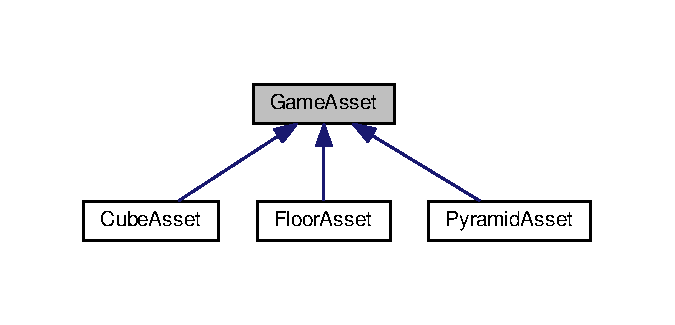
\includegraphics[width=324pt]{classGameAsset__inherit__graph}
\end{center}
\end{figure}
\subsection*{Public Member Functions}
\begin{DoxyCompactItemize}
\item 
virtual void \hyperlink{classGameAsset_a961aa51ca0a9961fc584c0b5d5431300}{Draw} (G\+Luint)=0
\end{DoxyCompactItemize}


\subsection{Member Function Documentation}
\hypertarget{classGameAsset_a961aa51ca0a9961fc584c0b5d5431300}{}\index{Game\+Asset@{Game\+Asset}!Draw@{Draw}}
\index{Draw@{Draw}!Game\+Asset@{Game\+Asset}}
\subsubsection[{Draw(\+G\+Luint)=0}]{\setlength{\rightskip}{0pt plus 5cm}virtual void Game\+Asset\+::\+Draw (
\begin{DoxyParamCaption}
\item[{G\+Luint}]{}
\end{DoxyParamCaption}
)\hspace{0.3cm}{\ttfamily [pure virtual]}}\label{classGameAsset_a961aa51ca0a9961fc584c0b5d5431300}


Implemented in \hyperlink{classCubeAsset_a1af568486056e254ffcf98fd99947bfe}{Cube\+Asset}, \hyperlink{classFloorAsset_a14650eb2c2cd75e990c351bad8636279}{Floor\+Asset}, and \hyperlink{classPyramidAsset_aaea45da4956d79ec9ab96e9d0ccef3fe}{Pyramid\+Asset}.



The documentation for this class was generated from the following file\+:\begin{DoxyCompactItemize}
\item 
src/\hyperlink{GameAsset_8h}{Game\+Asset.\+h}\end{DoxyCompactItemize}

\hypertarget{classGameAssetManager}{}\section{Game\+Asset\+Manager Class Reference}
\label{classGameAssetManager}\index{Game\+Asset\+Manager@{Game\+Asset\+Manager}}


\hyperlink{classGameAssetManager}{Game\+Asset\+Manager} is a container for Game\+Assets.  




{\ttfamily \#include $<$Game\+Asset\+Manager.\+h$>$}

\subsection*{Public Member Functions}
\begin{DoxyCompactItemize}
\item 
\hyperlink{classGameAssetManager_aaa0d58e276cc10ad91a7457085598a71}{Game\+Asset\+Manager} (\hyperlink{common_8h_add86e7c88dd109abea3f708b422f31f0}{Application\+Mode})
\begin{DoxyCompactList}\small\item\em Creates a \hyperlink{classGameAssetManager}{Game\+Asset\+Manager} to load the correct shaders based on the Application\+Mode. \end{DoxyCompactList}\item 
virtual \hyperlink{classGameAssetManager_a1270bd61ecbcca563f079803e40c9b77}{$\sim$\+Game\+Asset\+Manager} ()
\begin{DoxyCompactList}\small\item\em Deletes a \hyperlink{classGameAssetManager}{Game\+Asset\+Manager}, in particular it will clean up any modifications to the Open\+G\+L state. \end{DoxyCompactList}\item 
\hyperlink{classGameAssetManager_a2c9adcb72faa154c87eadc9bafe5269d}{Game\+Asset\+Manager} (\hyperlink{classGameAssetManager}{Game\+Asset\+Manager} const \&)
\begin{DoxyCompactList}\small\item\em Unimplemented copy constructor -- this means that the \hyperlink{classGameAssetManager}{Game\+Asset\+Manager} may not work as you\textquotesingle{}d expect when being copied. \end{DoxyCompactList}\item 
\hyperlink{classGameAssetManager_a44f6e2fd6b8ff1dd64e5697f1be7386d}{Game\+Asset\+Manager} (\hyperlink{classGameAssetManager}{Game\+Asset\+Manager} const \&\&)
\begin{DoxyCompactList}\small\item\em Unimplemented move constructor -- this unimplemented method violates the C++11 move semantics for \hyperlink{classGameAssetManager}{Game\+Asset\+Manager}. \end{DoxyCompactList}\item 
void \hyperlink{classGameAssetManager_ac72678a4ad5378c685aa6bae84a4e712}{operator=} (\hyperlink{classGameAssetManager}{Game\+Asset\+Manager} const \&)
\begin{DoxyCompactList}\small\item\em Unimplemented assisgnment operator -- violates the expected semantics for assignment in C++11. \end{DoxyCompactList}\item 
void \hyperlink{classGameAssetManager_ad3de8ff00d55ba04728b1de8213b2349}{Add\+Asset} (std\+::shared\+\_\+ptr$<$ \hyperlink{classGameAsset}{Game\+Asset} $>$)
\begin{DoxyCompactList}\small\item\em Adds a \hyperlink{classGameAsset}{Game\+Asset} to the scene graph. \end{DoxyCompactList}\item 
void \hyperlink{classGameAssetManager_a32837132bd70a9a9ed537323c2d3d886}{Draw} ()
\begin{DoxyCompactList}\small\item\em Draws each \hyperlink{classGameAsset}{Game\+Asset} in the scene graph. \end{DoxyCompactList}\end{DoxyCompactItemize}
\subsection*{Private Member Functions}
\begin{DoxyCompactItemize}
\item 
G\+Luint \hyperlink{classGameAssetManager_abec45b44a8b35ad2d7d817ba10e0dd8d}{Create\+G\+L\+Program} (std\+::string \&, std\+::string \&)
\begin{DoxyCompactList}\small\item\em When given the contents of a vertex shader and fragment shader \hyperlink{classGameAssetManager_abec45b44a8b35ad2d7d817ba10e0dd8d}{Game\+Asset\+Manager\+::\+Create\+G\+L\+Program} will compile and link them. \end{DoxyCompactList}\item 
G\+Luint \hyperlink{classGameAssetManager_a1a1e5c07f941e8d3fda40d9442ac7037}{Create\+G\+L\+E\+S\+Shader} (G\+Lenum, std\+::string \&)
\begin{DoxyCompactList}\small\item\em When given a type of shader to construct and the contents of a shader, \hyperlink{classGameAssetManager_a1a1e5c07f941e8d3fda40d9442ac7037}{Game\+Asset\+Manager\+::\+Create\+G\+L\+E\+S\+Shader} will create the shader or exit with error -\/1. \end{DoxyCompactList}\item 
std\+::pair$<$ G\+Lchar $\ast$, G\+Lint $>$ \hyperlink{classGameAssetManager_a23b124a213308a68a882727127601c97}{Read\+Shader} (std\+::string \&)
\begin{DoxyCompactList}\small\item\em Read\+Shader reads the contents of a file and packs it into a null termintated G\+Lchar $\ast$ which is suitable for sending to Open\+G\+L. \end{DoxyCompactList}\end{DoxyCompactItemize}
\subsection*{Private Attributes}
\begin{DoxyCompactItemize}
\item 
std\+::vector$<$ std\+::shared\+\_\+ptr$<$ \hyperlink{classGameAsset}{Game\+Asset} $>$ $>$ \hyperlink{classGameAssetManager_a671cddd92f1de4186c582fe0c4297b7d}{draw\+\_\+list}
\item 
G\+Luint \hyperlink{classGameAssetManager_ad7bab17862e06ca692289f934b40548b}{program\+\_\+token}
\end{DoxyCompactItemize}


\subsection{Detailed Description}
\hyperlink{classGameAssetManager}{Game\+Asset\+Manager} is a container for Game\+Assets. 

It also provides utility functions to to create a simple Open\+G\+L program that can be used to draw a simple \hyperlink{classGameAsset}{Game\+Asset}. 

\subsection{Constructor \& Destructor Documentation}
\hypertarget{classGameAssetManager_aaa0d58e276cc10ad91a7457085598a71}{}\index{Game\+Asset\+Manager@{Game\+Asset\+Manager}!Game\+Asset\+Manager@{Game\+Asset\+Manager}}
\index{Game\+Asset\+Manager@{Game\+Asset\+Manager}!Game\+Asset\+Manager@{Game\+Asset\+Manager}}
\subsubsection[{Game\+Asset\+Manager(\+Application\+Mode)}]{\setlength{\rightskip}{0pt plus 5cm}Game\+Asset\+Manager\+::\+Game\+Asset\+Manager (
\begin{DoxyParamCaption}
\item[{{\bf Application\+Mode}}]{mode}
\end{DoxyParamCaption}
)\hspace{0.3cm}{\ttfamily [explicit]}}\label{classGameAssetManager_aaa0d58e276cc10ad91a7457085598a71}


Creates a \hyperlink{classGameAssetManager}{Game\+Asset\+Manager} to load the correct shaders based on the Application\+Mode. 


\begin{DoxyCode}
7                                                        \{
8   std::string vertex\_shader(\textcolor{stringliteral}{"shaders/translate.vs"});
9   std::string fragment\_shader(\textcolor{stringliteral}{"shaders/fragment.fs"});
10 
11   \textcolor{keywordflow}{switch}(mode) \{
12   \textcolor{keywordflow}{case} \hyperlink{common_8h_add86e7c88dd109abea3f708b422f31f0a3dcfe0046eb5876e287dbf0914819b16}{ROTATE}:
13     vertex\_shader = \textcolor{stringliteral}{"shaders/rotate.vs"};
14     \textcolor{keywordflow}{break};
15   \textcolor{keywordflow}{case} \hyperlink{common_8h_add86e7c88dd109abea3f708b422f31f0a593be05a10070b4e7e0856e20590eaaf}{SCALE}:
16     vertex\_shader = \textcolor{stringliteral}{"shaders/scale.vs"};
17     \textcolor{keywordflow}{break};
18   \textcolor{keywordflow}{case} \hyperlink{common_8h_add86e7c88dd109abea3f708b422f31f0a25f73324dc93d9024c0c75b4e6815335}{TRANSFORM}:
19   \textcolor{keywordflow}{default}:
20     \textcolor{keywordflow}{break};
21   \};
22 
23   \hyperlink{classGameAssetManager_ad7bab17862e06ca692289f934b40548b}{program\_token} = \hyperlink{classGameAssetManager_abec45b44a8b35ad2d7d817ba10e0dd8d}{CreateGLProgram}(vertex\_shader, fragment\_shader);
24 \}
\end{DoxyCode}
\hypertarget{classGameAssetManager_a1270bd61ecbcca563f079803e40c9b77}{}\index{Game\+Asset\+Manager@{Game\+Asset\+Manager}!````~Game\+Asset\+Manager@{$\sim$\+Game\+Asset\+Manager}}
\index{````~Game\+Asset\+Manager@{$\sim$\+Game\+Asset\+Manager}!Game\+Asset\+Manager@{Game\+Asset\+Manager}}
\subsubsection[{$\sim$\+Game\+Asset\+Manager()}]{\setlength{\rightskip}{0pt plus 5cm}Game\+Asset\+Manager\+::$\sim$\+Game\+Asset\+Manager (
\begin{DoxyParamCaption}
{}
\end{DoxyParamCaption}
)\hspace{0.3cm}{\ttfamily [virtual]}}\label{classGameAssetManager_a1270bd61ecbcca563f079803e40c9b77}


Deletes a \hyperlink{classGameAssetManager}{Game\+Asset\+Manager}, in particular it will clean up any modifications to the Open\+G\+L state. 


\begin{DoxyCode}
30                                     \{
31   glDeleteProgram(\hyperlink{classGameAssetManager_ad7bab17862e06ca692289f934b40548b}{program\_token});
32 \}
\end{DoxyCode}
\hypertarget{classGameAssetManager_a2c9adcb72faa154c87eadc9bafe5269d}{}\index{Game\+Asset\+Manager@{Game\+Asset\+Manager}!Game\+Asset\+Manager@{Game\+Asset\+Manager}}
\index{Game\+Asset\+Manager@{Game\+Asset\+Manager}!Game\+Asset\+Manager@{Game\+Asset\+Manager}}
\subsubsection[{Game\+Asset\+Manager(\+Game\+Asset\+Manager const \&)}]{\setlength{\rightskip}{0pt plus 5cm}Game\+Asset\+Manager\+::\+Game\+Asset\+Manager (
\begin{DoxyParamCaption}
\item[{{\bf Game\+Asset\+Manager} const \&}]{the\+\_\+manager}
\end{DoxyParamCaption}
)}\label{classGameAssetManager_a2c9adcb72faa154c87eadc9bafe5269d}


Unimplemented copy constructor -- this means that the \hyperlink{classGameAssetManager}{Game\+Asset\+Manager} may not work as you\textquotesingle{}d expect when being copied. 


\begin{DoxyCode}
38                                                                       \{
39   \textcolor{comment}{// TODO: implement this}
40 \}
\end{DoxyCode}
\hypertarget{classGameAssetManager_a44f6e2fd6b8ff1dd64e5697f1be7386d}{}\index{Game\+Asset\+Manager@{Game\+Asset\+Manager}!Game\+Asset\+Manager@{Game\+Asset\+Manager}}
\index{Game\+Asset\+Manager@{Game\+Asset\+Manager}!Game\+Asset\+Manager@{Game\+Asset\+Manager}}
\subsubsection[{Game\+Asset\+Manager(\+Game\+Asset\+Manager const \&\&)}]{\setlength{\rightskip}{0pt plus 5cm}Game\+Asset\+Manager\+::\+Game\+Asset\+Manager (
\begin{DoxyParamCaption}
\item[{{\bf Game\+Asset\+Manager} const \&\&}]{the\+\_\+manager}
\end{DoxyParamCaption}
)}\label{classGameAssetManager_a44f6e2fd6b8ff1dd64e5697f1be7386d}


Unimplemented move constructor -- this unimplemented method violates the C++11 move semantics for \hyperlink{classGameAssetManager}{Game\+Asset\+Manager}. 


\begin{DoxyCode}
46                                                                        \{
47   \textcolor{comment}{// TODO: implement this}
48 \}
\end{DoxyCode}


\subsection{Member Function Documentation}
\hypertarget{classGameAssetManager_ad3de8ff00d55ba04728b1de8213b2349}{}\index{Game\+Asset\+Manager@{Game\+Asset\+Manager}!Add\+Asset@{Add\+Asset}}
\index{Add\+Asset@{Add\+Asset}!Game\+Asset\+Manager@{Game\+Asset\+Manager}}
\subsubsection[{Add\+Asset(std\+::shared\+\_\+ptr$<$ Game\+Asset $>$)}]{\setlength{\rightskip}{0pt plus 5cm}void Game\+Asset\+Manager\+::\+Add\+Asset (
\begin{DoxyParamCaption}
\item[{std\+::shared\+\_\+ptr$<$ {\bf Game\+Asset} $>$}]{the\+\_\+asset}
\end{DoxyParamCaption}
)}\label{classGameAssetManager_ad3de8ff00d55ba04728b1de8213b2349}


Adds a \hyperlink{classGameAsset}{Game\+Asset} to the scene graph. 


\begin{DoxyCode}
61                                                                   \{
62   \hyperlink{classGameAssetManager_a671cddd92f1de4186c582fe0c4297b7d}{draw\_list}.push\_back(the\_asset);
63 \}
\end{DoxyCode}
\hypertarget{classGameAssetManager_a1a1e5c07f941e8d3fda40d9442ac7037}{}\index{Game\+Asset\+Manager@{Game\+Asset\+Manager}!Create\+G\+L\+E\+S\+Shader@{Create\+G\+L\+E\+S\+Shader}}
\index{Create\+G\+L\+E\+S\+Shader@{Create\+G\+L\+E\+S\+Shader}!Game\+Asset\+Manager@{Game\+Asset\+Manager}}
\subsubsection[{Create\+G\+L\+E\+S\+Shader(\+G\+Lenum, std\+::string \&)}]{\setlength{\rightskip}{0pt plus 5cm}G\+Luint Game\+Asset\+Manager\+::\+Create\+G\+L\+E\+S\+Shader (
\begin{DoxyParamCaption}
\item[{G\+Lenum}]{type, }
\item[{std\+::string \&}]{shader}
\end{DoxyParamCaption}
)\hspace{0.3cm}{\ttfamily [private]}}\label{classGameAssetManager_a1a1e5c07f941e8d3fda40d9442ac7037}


When given a type of shader to construct and the contents of a shader, \hyperlink{classGameAssetManager_a1a1e5c07f941e8d3fda40d9442ac7037}{Game\+Asset\+Manager\+::\+Create\+G\+L\+E\+S\+Shader} will create the shader or exit with error -\/1. 

\begin{DoxyReturn}{Returns}
the G\+L \char`\"{}token\char`\"{} for the requested shader. 
\end{DoxyReturn}

\begin{DoxyCode}
110                                                                          \{
111   GLuint shader\_token;
112   GLint shader\_ok;
113   \textcolor{keyword}{auto} source = \hyperlink{classGameAssetManager_a23b124a213308a68a882727127601c97}{ReadShader}(shader);
114 
115   \textcolor{keywordflow}{if} (!source.first)
116     \textcolor{keywordflow}{return} 0;
117 
118   shader\_token = glCreateShader(type);
119   glShaderSource(shader\_token, 1, (\textcolor{keyword}{const} GLchar**)&source.first, &source.second);
120   glCompileShader(shader\_token);
121   \textcolor{keyword}{delete}(source.first);
122 
123   glGetShaderiv(shader\_token, GL\_COMPILE\_STATUS, &shader\_ok);
124   \textcolor{keywordflow}{if} (!shader\_ok) \{
125     GLint maxLength = 0;
126     glGetShaderiv(shader\_token, GL\_INFO\_LOG\_LENGTH, &maxLength);
127 
128     \textcolor{comment}{//The maxLength includes the NULL character}
129     std::vector<char> errorLog(maxLength);
130     glGetShaderInfoLog(shader\_token, maxLength, &maxLength, &errorLog[0]);
131 
132     \textcolor{comment}{//Provide the infolog in whatever manor you deem best.}
133     std::cerr << \textcolor{stringliteral}{"Failed to compile "} << shader << \textcolor{stringliteral}{" with error code "} << shader\_ok << std::endl;
134     \textcolor{keywordflow}{for}(\textcolor{keyword}{auto} c: errorLog) \{
135       std::cerr << c;
136     \}
137 
138     glDeleteShader(shader\_token); \textcolor{comment}{//Don't leak the shader.}
139     exit(-1);
140   \}
141   \textcolor{keywordflow}{return} shader\_token;
142 \}
\end{DoxyCode}
\hypertarget{classGameAssetManager_abec45b44a8b35ad2d7d817ba10e0dd8d}{}\index{Game\+Asset\+Manager@{Game\+Asset\+Manager}!Create\+G\+L\+Program@{Create\+G\+L\+Program}}
\index{Create\+G\+L\+Program@{Create\+G\+L\+Program}!Game\+Asset\+Manager@{Game\+Asset\+Manager}}
\subsubsection[{Create\+G\+L\+Program(std\+::string \&, std\+::string \&)}]{\setlength{\rightskip}{0pt plus 5cm}G\+Luint Game\+Asset\+Manager\+::\+Create\+G\+L\+Program (
\begin{DoxyParamCaption}
\item[{std\+::string \&}]{vertex\+\_\+shader, }
\item[{std\+::string \&}]{fragment\+\_\+shader}
\end{DoxyParamCaption}
)\hspace{0.3cm}{\ttfamily [private]}}\label{classGameAssetManager_abec45b44a8b35ad2d7d817ba10e0dd8d}


When given the contents of a vertex shader and fragment shader \hyperlink{classGameAssetManager_abec45b44a8b35ad2d7d817ba10e0dd8d}{Game\+Asset\+Manager\+::\+Create\+G\+L\+Program} will compile and link them. 

This implementation will exit with -\/1 error if an error is detected.

\begin{DoxyReturn}{Returns}
the G\+L \char`\"{}token\char`\"{} referring to the gl program. 
\end{DoxyReturn}

\begin{DoxyCode}
82                                                                         \{
83   \textcolor{keyword}{auto} v\_shader\_token = \hyperlink{classGameAssetManager_a1a1e5c07f941e8d3fda40d9442ac7037}{CreateGLESShader}(GL\_VERTEX\_SHADER, vertex\_shader);
84   \textcolor{keyword}{auto} f\_shader\_token = \hyperlink{classGameAssetManager_a1a1e5c07f941e8d3fda40d9442ac7037}{CreateGLESShader}(GL\_FRAGMENT\_SHADER, fragment\_shader);
85 
86   GLint program\_ok;
87 
88   GLuint program = glCreateProgram();
89 
90   glAttachShader(program, v\_shader\_token);
91   glAttachShader(program, f\_shader\_token);
92   glLinkProgram(program);
93 
94   glGetProgramiv(program, GL\_LINK\_STATUS, &program\_ok);
95   \textcolor{keywordflow}{if} (!program\_ok) \{
96     std::cerr << \textcolor{stringliteral}{"Failed to link shader program:"} << std::endl;
97     glDeleteProgram(program);
98     exit(-1);
99   \}
100   \textcolor{keywordflow}{return} program;
101 \}
\end{DoxyCode}
\hypertarget{classGameAssetManager_a32837132bd70a9a9ed537323c2d3d886}{}\index{Game\+Asset\+Manager@{Game\+Asset\+Manager}!Draw@{Draw}}
\index{Draw@{Draw}!Game\+Asset\+Manager@{Game\+Asset\+Manager}}
\subsubsection[{Draw()}]{\setlength{\rightskip}{0pt plus 5cm}void Game\+Asset\+Manager\+::\+Draw (
\begin{DoxyParamCaption}
{}
\end{DoxyParamCaption}
)}\label{classGameAssetManager_a32837132bd70a9a9ed537323c2d3d886}


Draws each \hyperlink{classGameAsset}{Game\+Asset} in the scene graph. 


\begin{DoxyCode}
68                             \{
69   \textcolor{keywordflow}{for}(\textcolor{keyword}{auto} ga: \hyperlink{classGameAssetManager_a671cddd92f1de4186c582fe0c4297b7d}{draw\_list}) \{
70     ga->Draw(\hyperlink{classGameAssetManager_ad7bab17862e06ca692289f934b40548b}{program\_token});
71   \}
72 \}
\end{DoxyCode}
\hypertarget{classGameAssetManager_ac72678a4ad5378c685aa6bae84a4e712}{}\index{Game\+Asset\+Manager@{Game\+Asset\+Manager}!operator=@{operator=}}
\index{operator=@{operator=}!Game\+Asset\+Manager@{Game\+Asset\+Manager}}
\subsubsection[{operator=(\+Game\+Asset\+Manager const \&)}]{\setlength{\rightskip}{0pt plus 5cm}void Game\+Asset\+Manager\+::operator= (
\begin{DoxyParamCaption}
\item[{{\bf Game\+Asset\+Manager} const \&}]{the\+\_\+manager}
\end{DoxyParamCaption}
)}\label{classGameAssetManager_ac72678a4ad5378c685aa6bae84a4e712}


Unimplemented assisgnment operator -- violates the expected semantics for assignment in C++11. 


\begin{DoxyCode}
54                                                                     \{
55   \textcolor{comment}{// TODO: implement this}
56 \}
\end{DoxyCode}
\hypertarget{classGameAssetManager_a23b124a213308a68a882727127601c97}{}\index{Game\+Asset\+Manager@{Game\+Asset\+Manager}!Read\+Shader@{Read\+Shader}}
\index{Read\+Shader@{Read\+Shader}!Game\+Asset\+Manager@{Game\+Asset\+Manager}}
\subsubsection[{Read\+Shader(std\+::string \&)}]{\setlength{\rightskip}{0pt plus 5cm}std\+::pair$<$ G\+Lchar $\ast$, G\+Lint $>$ Game\+Asset\+Manager\+::\+Read\+Shader (
\begin{DoxyParamCaption}
\item[{std\+::string \&}]{shader}
\end{DoxyParamCaption}
)\hspace{0.3cm}{\ttfamily [private]}}\label{classGameAssetManager_a23b124a213308a68a882727127601c97}


Read\+Shader reads the contents of a file and packs it into a null termintated G\+Lchar $\ast$ which is suitable for sending to Open\+G\+L. 

\begin{DoxyReturn}{Returns}
a pair consisting of the shader file contents and a holder for the Open\+G\+L \char`\"{}token\char`\"{}. 
\end{DoxyReturn}

\begin{DoxyCode}
151                                                                         \{
152   std::ifstream input\_file;
153   GLint length;
154   input\_file.open(shader, std::ios::in);
155 
156   input\_file.seekg(0, std::ios::end);  \textcolor{comment}{// go to the end of the file}
157   length = input\_file.tellg();    \textcolor{comment}{// get length of the file}
158   input\_file.seekg(0, std::ios::beg);  \textcolor{comment}{// go to beginning of the file}
159 
160   GLchar * buffer = \textcolor{keyword}{new} GLchar[length+1];
161   input\_file.read(buffer, length);
162   buffer[length+1]=\textcolor{charliteral}{'\(\backslash\)0'};  \textcolor{comment}{// Ensure null terminated}
163 
164   input\_file.close();
165   \textcolor{keywordflow}{return} std::make\_pair(buffer, length);
166 \}
\end{DoxyCode}


\subsection{Member Data Documentation}
\hypertarget{classGameAssetManager_a671cddd92f1de4186c582fe0c4297b7d}{}\index{Game\+Asset\+Manager@{Game\+Asset\+Manager}!draw\+\_\+list@{draw\+\_\+list}}
\index{draw\+\_\+list@{draw\+\_\+list}!Game\+Asset\+Manager@{Game\+Asset\+Manager}}
\subsubsection[{draw\+\_\+list}]{\setlength{\rightskip}{0pt plus 5cm}std\+::vector$<$std\+::shared\+\_\+ptr$<${\bf Game\+Asset}$>$ $>$ Game\+Asset\+Manager\+::draw\+\_\+list\hspace{0.3cm}{\ttfamily [private]}}\label{classGameAssetManager_a671cddd92f1de4186c582fe0c4297b7d}
\hypertarget{classGameAssetManager_ad7bab17862e06ca692289f934b40548b}{}\index{Game\+Asset\+Manager@{Game\+Asset\+Manager}!program\+\_\+token@{program\+\_\+token}}
\index{program\+\_\+token@{program\+\_\+token}!Game\+Asset\+Manager@{Game\+Asset\+Manager}}
\subsubsection[{program\+\_\+token}]{\setlength{\rightskip}{0pt plus 5cm}G\+Luint Game\+Asset\+Manager\+::program\+\_\+token\hspace{0.3cm}{\ttfamily [private]}}\label{classGameAssetManager_ad7bab17862e06ca692289f934b40548b}


The documentation for this class was generated from the following files\+:\begin{DoxyCompactItemize}
\item 
src/\hyperlink{GameAssetManager_8h}{Game\+Asset\+Manager.\+h}\item 
src/\hyperlink{GameAssetManager_8cc}{Game\+Asset\+Manager.\+cc}\end{DoxyCompactItemize}

\hypertarget{classGameWorld}{}\section{Game\+World Class Reference}
\label{classGameWorld}\index{Game\+World@{Game\+World}}


\hyperlink{classGameWorld}{Game\+World} allows us to separate the management of the game world from the nuts and bolts of game loop initialisation.  




{\ttfamily \#include $<$Game\+World.\+h$>$}

\subsection*{Public Member Functions}
\begin{DoxyCompactItemize}
\item 
\hyperlink{classGameWorld_a17a84e57a80600961088afc753036f89}{Game\+World} (\hyperlink{common_8h_add86e7c88dd109abea3f708b422f31f0}{Application\+Mode})
\begin{DoxyCompactList}\small\item\em We thread the Application\+Mode through the \hyperlink{classGameWorld}{Game\+World} ss we want to read it in from the user. \end{DoxyCompactList}\item 
void \hyperlink{classGameWorld_a275418607d8286979b276f165ad5876b}{Draw} ()
\begin{DoxyCompactList}\small\item\em Calling \hyperlink{classGameWorld_a275418607d8286979b276f165ad5876b}{Draw()} will draw the entire world. \end{DoxyCompactList}\end{DoxyCompactItemize}
\subsection*{Private Attributes}
\begin{DoxyCompactItemize}
\item 
std\+::shared\+\_\+ptr$<$ \hyperlink{classGameAssetManager}{Game\+Asset\+Manager} $>$ \hyperlink{classGameWorld_aec5c0bca4fb5a41e4aac2dce2871266d}{asset\+\_\+manager}
\end{DoxyCompactItemize}


\subsection{Detailed Description}
\hyperlink{classGameWorld}{Game\+World} allows us to separate the management of the game world from the nuts and bolts of game loop initialisation. 

The \hyperlink{classGameWorld}{Game\+World} currently has a very simplified scene graph consisiting of a single \hyperlink{classGameAssetManager}{Game\+Asset\+Manager}. 

\subsection{Constructor \& Destructor Documentation}
\hypertarget{classGameWorld_a17a84e57a80600961088afc753036f89}{}\index{Game\+World@{Game\+World}!Game\+World@{Game\+World}}
\index{Game\+World@{Game\+World}!Game\+World@{Game\+World}}
\subsubsection[{Game\+World(\+Application\+Mode)}]{\setlength{\rightskip}{0pt plus 5cm}Game\+World\+::\+Game\+World (
\begin{DoxyParamCaption}
\item[{{\bf Application\+Mode}}]{mode}
\end{DoxyParamCaption}
)}\label{classGameWorld_a17a84e57a80600961088afc753036f89}


We thread the Application\+Mode through the \hyperlink{classGameWorld}{Game\+World} ss we want to read it in from the user. 

Threading the state through the various function calls is preferable (in this case) to having some kind of global state. Cube spawning with Array Using a 2\+D array to spawn multiple voxels 1 -\/ Floor piece 2 -\/ Floor piece and cube 3 -\/ Floor piece and pyramid

Spawning Floor floor is spawned with; X offset equal to the half of the x plane so the positions are roughly center Y is a constant as the floor is one flat plane Z is determined by the Y value

Spawning Cubes Spawns floor asset and a Cube asset

Spawning Pyramids Spawns floor asset and a Pyramid asset above it
\begin{DoxyCode}
5                                           : \hyperlink{classGameWorld_aec5c0bca4fb5a41e4aac2dce2871266d}{asset\_manager} (make\_shared<GameAssetManager>(mode)
      )\{
6 
14 
15 \textcolor{keywordtype}{int} X,Y;
16 \textcolor{keywordtype}{int} Z = -1;
17 \textcolor{keywordtype}{int} planeX = 12;
18 \textcolor{keywordtype}{int} planeY = 12;
19 
20 \textcolor{keywordtype}{int} plane[planeX][planeY] = \{
21 \{1, 1, 1, 1, 1, 1, 1, 1, 1, 1, 1, 1\},
22 \{1, 1, 1, 1, 1, 1, 1, 1, 1, 1, 1, 1\},
23 \{1, 1, 1, 1, 1, 1, 1, 1, 1, 1, 1, 1\},
24 \{1, 1, 1, 1, 1, 1, 1, 1, 1, 1, 1, 1\},
25 \{1, 1, 1, 1, 1, 1, 1, 1, 1, 2, 1, 1\},
26 \{1, 1, 1, 1, 1, 1, 1, 1, 1, 1, 1, 1\},
27 \{1, 1, 1, 1, 1, 1, 1, 1, 1, 1, 1, 1\},
28 \{1, 1, 1, 1, 1, 1, 1, 3, 1, 1, 1, 1\},
29 \{1, 1, 1, 2, 1, 1, 1, 1, 1, 1, 1, 3\},
30 \{1, 1, 1, 1, 1, 1, 1, 1, 1, 1, 1, 1\},
31 \{1, 3, 1, 1, 1, 1, 1, 1, 1, 1, 1, 1\},
32 \{1, 1, 1, 1, 1, 1, 1, 1, 1, 1, 1, 1\},
33 \};
34 
42 
43  \textcolor{keywordflow}{for}( X=0; X<planeX; X++)\{
44    \textcolor{keywordflow}{for} (Y=0; Y<planeY; Y++)\{
45     \textcolor{keywordflow}{if}( plane[Y][X] == 1)\{  
46      \hyperlink{classGameWorld_aec5c0bca4fb5a41e4aac2dce2871266d}{asset\_manager}->AddAsset(make\_shared<FloorAsset>((X)-(planeX/2),-6.00f,(Z*Y)));
47     \}    
48 
53     \textcolor{keywordflow}{else} \textcolor{keywordflow}{if}( plane[Y][X] == 2)\{
54       \hyperlink{classGameWorld_aec5c0bca4fb5a41e4aac2dce2871266d}{asset\_manager}->AddAsset(make\_shared<FloorAsset>((X)-(planeX/2),-6.00f,(Z*Y)));
55       \hyperlink{classGameWorld_aec5c0bca4fb5a41e4aac2dce2871266d}{asset\_manager}->AddAsset(make\_shared<CubeAsset>((X)-(planeX/2),2.00f,(Z*Y)));
56 
57     \}
62     \textcolor{keywordflow}{else} \textcolor{keywordflow}{if}( plane[Y][X] == 3)\{
63       \hyperlink{classGameWorld_aec5c0bca4fb5a41e4aac2dce2871266d}{asset\_manager}->AddAsset(make\_shared<FloorAsset>((X)-(planeX/2),-6.00f,(Z*Y)));
64       \hyperlink{classGameWorld_aec5c0bca4fb5a41e4aac2dce2871266d}{asset\_manager}->AddAsset(make\_shared<PyramidAsset>((X)-(planeX/2),3.00f,(Z*Y)));
65     \}
66   \}
67  \}
68 
69 \}
\end{DoxyCode}


\subsection{Member Function Documentation}
\hypertarget{classGameWorld_a275418607d8286979b276f165ad5876b}{}\index{Game\+World@{Game\+World}!Draw@{Draw}}
\index{Draw@{Draw}!Game\+World@{Game\+World}}
\subsubsection[{Draw()}]{\setlength{\rightskip}{0pt plus 5cm}void Game\+World\+::\+Draw (
\begin{DoxyParamCaption}
{}
\end{DoxyParamCaption}
)}\label{classGameWorld_a275418607d8286979b276f165ad5876b}


Calling \hyperlink{classGameWorld_a275418607d8286979b276f165ad5876b}{Draw()} will draw the entire world. 


\begin{DoxyCode}
71                      \{
72   \hyperlink{classGameWorld_aec5c0bca4fb5a41e4aac2dce2871266d}{asset\_manager}->Draw();
73 \}
\end{DoxyCode}


\subsection{Member Data Documentation}
\hypertarget{classGameWorld_aec5c0bca4fb5a41e4aac2dce2871266d}{}\index{Game\+World@{Game\+World}!asset\+\_\+manager@{asset\+\_\+manager}}
\index{asset\+\_\+manager@{asset\+\_\+manager}!Game\+World@{Game\+World}}
\subsubsection[{asset\+\_\+manager}]{\setlength{\rightskip}{0pt plus 5cm}std\+::shared\+\_\+ptr$<${\bf Game\+Asset\+Manager}$>$ Game\+World\+::asset\+\_\+manager\hspace{0.3cm}{\ttfamily [private]}}\label{classGameWorld_aec5c0bca4fb5a41e4aac2dce2871266d}


The documentation for this class was generated from the following files\+:\begin{DoxyCompactItemize}
\item 
src/\hyperlink{GameWorld_8h}{Game\+World.\+h}\item 
src/\hyperlink{GameWorld_8cc}{Game\+World.\+cc}\end{DoxyCompactItemize}

\hypertarget{classPyramidAsset}{}\section{Pyramid\+Asset Class Reference}
\label{classPyramidAsset}\index{Pyramid\+Asset@{Pyramid\+Asset}}


{\ttfamily \#include $<$Pyramid\+Asset.\+h$>$}



Inheritance diagram for Pyramid\+Asset\+:
% FIG 0


Collaboration diagram for Pyramid\+Asset\+:
% FIG 1
\subsection*{Public Member Functions}
\begin{DoxyCompactItemize}
\item 
\hyperlink{classPyramidAsset_a3f7c6fd658ed0d3e276d7fe6c1de95d1}{Pyramid\+Asset} (G\+Lfloat x, G\+Lfloat y, G\+Lfloat z)
\item 
\hyperlink{classPyramidAsset_afb388a196f43a3808b2d4f6fdb89ee84}{$\sim$\+Pyramid\+Asset} ()
\item 
virtual void \hyperlink{classPyramidAsset_aaea45da4956d79ec9ab96e9d0ccef3fe}{Draw} (G\+Luint)
\end{DoxyCompactItemize}
\subsection*{Private Member Functions}
\begin{DoxyCompactItemize}
\item 
void \hyperlink{classPyramidAsset_a34350044042e0098446dc9e0a260cb70}{check\+Error} (std\+::string file, int line)
\end{DoxyCompactItemize}
\subsection*{Private Attributes}
\begin{DoxyCompactItemize}
\item 
G\+Luint \hyperlink{classPyramidAsset_a5566105859271b493eab3b5f9c02f866}{element\+\_\+buffer\+\_\+length}
\item 
G\+Luint \hyperlink{classPyramidAsset_ae576f67cdec51a52645131919d86a38a}{color\+\_\+buffer\+\_\+length}
\item 
G\+Luint \hyperlink{classPyramidAsset_a9252f29d7dc33374d43dd779db4fcce4}{vertex\+\_\+buffer\+\_\+length}
\item 
G\+Luint \hyperlink{classPyramidAsset_a54d9cec42bc77d07a66e6c1cd55049b0}{vertex\+\_\+buffer\+\_\+token}
\item 
G\+Luint \hyperlink{classPyramidAsset_a7a984ee57fa7deda5aedf8b1f5f85c6f}{color\+\_\+buffer\+\_\+token}
\item 
G\+Luint \hyperlink{classPyramidAsset_a6f7e2f50904d2941e33df8eb7f5f9c2d}{element\+\_\+buffer\+\_\+token}
\end{DoxyCompactItemize}


\subsection{Constructor \& Destructor Documentation}
\hypertarget{classPyramidAsset_a3f7c6fd658ed0d3e276d7fe6c1de95d1}{}\index{Pyramid\+Asset@{Pyramid\+Asset}!Pyramid\+Asset@{Pyramid\+Asset}}
\index{Pyramid\+Asset@{Pyramid\+Asset}!Pyramid\+Asset@{Pyramid\+Asset}}
\subsubsection[{Pyramid\+Asset(\+G\+Lfloat x, G\+Lfloat y, G\+Lfloat z)}]{\setlength{\rightskip}{0pt plus 5cm}Pyramid\+Asset\+::\+Pyramid\+Asset (
\begin{DoxyParamCaption}
\item[{G\+Lfloat}]{x, }
\item[{G\+Lfloat}]{y, }
\item[{G\+Lfloat}]{z}
\end{DoxyParamCaption}
)}\label{classPyramidAsset_a3f7c6fd658ed0d3e276d7fe6c1de95d1}
Pyramid Creation models coordinates, origin dependant on xyz variables. vertex buffer models coordinates, for the triangles. colour buffer models the colour of the object triangles. element buffer creates the cube using 6 triangles.
\begin{DoxyCode}
3                                                           \{
4 
12 
13   GLfloat vertex\_buffer [] \{
14       -0.5f + x,  0.0f + y, -0.5f + z   \textcolor{comment}{//0}
15     , -0.5f + x,  0.0f + y,  0.5f + z   \textcolor{comment}{//1}
16     ,  0.5f + x,  0.0f + y, -0.5f + z   \textcolor{comment}{//2}
17     ,  0.5f + x,  0.0f + y,  0.5f + z   \textcolor{comment}{//3}
18     ,  0.0f + x,  1.0f + y,  0.0f + z   \textcolor{comment}{//4}
19   \};
20   \hyperlink{classPyramidAsset_a9252f29d7dc33374d43dd779db4fcce4}{vertex\_buffer\_length} = \textcolor{keyword}{sizeof}(vertex\_buffer);
21 
22   GLfloat color\_buffer [] \{
23       1.000f, 0.000f, 0.000f \textcolor{comment}{//0}
24     , 1.000f, 0.000f, 0.000f \textcolor{comment}{//1}
25     , 1.000f, 0.000f, 0.000f \textcolor{comment}{//2}
26     , 1.000f, 0.000f, 0.000f \textcolor{comment}{//3}
27     , 1.000f, 0.000f, 0.000f \textcolor{comment}{//4}
28   \};
29   \hyperlink{classPyramidAsset_ae576f67cdec51a52645131919d86a38a}{color\_buffer\_length} = \textcolor{keyword}{sizeof}(color\_buffer);
30 
31   GLuint element\_buffer []  \{
32       1, 4, 0  \textcolor{comment}{// left}
33     , 0, 4, 2  \textcolor{comment}{// front}
34     , 2, 4, 3  \textcolor{comment}{// right}
35     , 1, 4, 3  \textcolor{comment}{// back}
36     , 0, 1, 2  \textcolor{comment}{// bottom}
37     , 1, 3, 2     
38   \};
39   \hyperlink{classPyramidAsset_a5566105859271b493eab3b5f9c02f866}{element\_buffer\_length} = \textcolor{keyword}{sizeof}(element\_buffer);
40   \textcolor{comment}{// Transfer buffers to the GPU}
41   \textcolor{comment}{//}
42 
43   \textcolor{comment}{// create vertex buffer}
44   glGenBuffers(1, &\hyperlink{classPyramidAsset_a54d9cec42bc77d07a66e6c1cd55049b0}{vertex\_buffer\_token});
45   \textcolor{comment}{// immediately bind the buffer and transfer the data}
46   glBindBuffer(GL\_ARRAY\_BUFFER, \hyperlink{classPyramidAsset_a54d9cec42bc77d07a66e6c1cd55049b0}{vertex\_buffer\_token});
47   glBufferData(GL\_ARRAY\_BUFFER, \hyperlink{classPyramidAsset_a9252f29d7dc33374d43dd779db4fcce4}{vertex\_buffer\_length}, vertex\_buffer, GL\_STATIC\_DRAW);
48 
49   \textcolor{comment}{// create color buffer}
50   glGenBuffers(1, &\hyperlink{classPyramidAsset_a7a984ee57fa7deda5aedf8b1f5f85c6f}{color\_buffer\_token});
51   \textcolor{comment}{// immediately bind the buffer and transfer the data}
52   glBindBuffer(GL\_ARRAY\_BUFFER, \hyperlink{classPyramidAsset_a7a984ee57fa7deda5aedf8b1f5f85c6f}{color\_buffer\_token});
53   glBufferData(GL\_ARRAY\_BUFFER, \hyperlink{classPyramidAsset_ae576f67cdec51a52645131919d86a38a}{color\_buffer\_length}, color\_buffer, GL\_STATIC\_DRAW);
54   
55   glGenBuffers(1, &\hyperlink{classPyramidAsset_a6f7e2f50904d2941e33df8eb7f5f9c2d}{element\_buffer\_token});
56   glBindBuffer(GL\_ELEMENT\_ARRAY\_BUFFER, \hyperlink{classPyramidAsset_a6f7e2f50904d2941e33df8eb7f5f9c2d}{element\_buffer\_token});
57   glBufferData(GL\_ELEMENT\_ARRAY\_BUFFER, \hyperlink{classPyramidAsset_a5566105859271b493eab3b5f9c02f866}{element\_buffer\_length}, element\_buffer, 
      GL\_STATIC\_DRAW);
58 \}
\end{DoxyCode}
\hypertarget{classPyramidAsset_afb388a196f43a3808b2d4f6fdb89ee84}{}\index{Pyramid\+Asset@{Pyramid\+Asset}!````~Pyramid\+Asset@{$\sim$\+Pyramid\+Asset}}
\index{````~Pyramid\+Asset@{$\sim$\+Pyramid\+Asset}!Pyramid\+Asset@{Pyramid\+Asset}}
\subsubsection[{$\sim$\+Pyramid\+Asset()}]{\setlength{\rightskip}{0pt plus 5cm}Pyramid\+Asset\+::$\sim$\+Pyramid\+Asset (
\begin{DoxyParamCaption}
{}
\end{DoxyParamCaption}
)}\label{classPyramidAsset_afb388a196f43a3808b2d4f6fdb89ee84}

\begin{DoxyCode}
60                             \{
61 \}
\end{DoxyCode}


\subsection{Member Function Documentation}
\hypertarget{classPyramidAsset_a34350044042e0098446dc9e0a260cb70}{}\index{Pyramid\+Asset@{Pyramid\+Asset}!check\+Error@{check\+Error}}
\index{check\+Error@{check\+Error}!Pyramid\+Asset@{Pyramid\+Asset}}
\subsubsection[{check\+Error(std\+::string file, int line)}]{\setlength{\rightskip}{0pt plus 5cm}void Pyramid\+Asset\+::check\+Error (
\begin{DoxyParamCaption}
\item[{std\+::string}]{file, }
\item[{int}]{line}
\end{DoxyParamCaption}
)\hspace{0.3cm}{\ttfamily [private]}}\label{classPyramidAsset_a34350044042e0098446dc9e0a260cb70}

\begin{DoxyCode}
70                                                       \{
71   GLenum gl\_error = glGetError();
72   \textcolor{keywordflow}{if}(GL\_NO\_ERROR != gl\_error) \{
73     std::cerr << \textcolor{stringliteral}{"GL error in "} << file << \textcolor{stringliteral}{" at line "} << line << \textcolor{stringliteral}{" error: "} << gl\_error << std::endl;
74     exit(-1);
75   \}
76 \}
\end{DoxyCode}
\hypertarget{classPyramidAsset_aaea45da4956d79ec9ab96e9d0ccef3fe}{}\index{Pyramid\+Asset@{Pyramid\+Asset}!Draw@{Draw}}
\index{Draw@{Draw}!Pyramid\+Asset@{Pyramid\+Asset}}
\subsubsection[{Draw(\+G\+Luint)}]{\setlength{\rightskip}{0pt plus 5cm}void Pyramid\+Asset\+::\+Draw (
\begin{DoxyParamCaption}
\item[{G\+Luint}]{program\+\_\+token}
\end{DoxyParamCaption}
)\hspace{0.3cm}{\ttfamily [virtual]}}\label{classPyramidAsset_aaea45da4956d79ec9ab96e9d0ccef3fe}
repeated buffer array for color buffer

Implements \hyperlink{classGameAsset_a961aa51ca0a9961fc584c0b5d5431300}{Game\+Asset}.


\begin{DoxyCode}
78                                             \{
79   \textcolor{keywordflow}{if}(!glIsProgram(program\_token)) \{
80     std::cerr << \textcolor{stringliteral}{"Drawing Pyramid with invalid program"} << std::endl;
81     \textcolor{keywordflow}{return};
82   \}
83   GLint validation\_ok;
84   glValidateProgram(program\_token);
85   glGetProgramiv(program\_token, GL\_VALIDATE\_STATUS, &validation\_ok);
86   \textcolor{keywordflow}{if}(!validation\_ok) \{
87     GLint maxLength = 0;
88     glGetProgramiv(program\_token, GL\_INFO\_LOG\_LENGTH, &maxLength);
89 
90     \textcolor{comment}{//The maxLength includes the NULL character}
91     std::vector<char> errorLog(maxLength);
92     glGetProgramInfoLog(program\_token, maxLength, &maxLength, &errorLog[0]);
93 
94     std::cerr << \textcolor{stringliteral}{"Invalid program "} << program\_token << \textcolor{stringliteral}{" with error code "} << validation\_ok << std::endl;
95     \textcolor{keywordflow}{for}(\textcolor{keyword}{auto} c: errorLog) \{
96       std::cerr << c;
97     \}
98     exit(-1);
99   \}
100 
101   GLuint position\_attrib = glGetAttribLocation(program\_token, \textcolor{stringliteral}{"position"});
102   \hyperlink{PyramidAsset_8cc_a75f201b0e53e68726854997957322b8d}{checkGLError}();
103 
104   glUseProgram(program\_token);
105   \hyperlink{PyramidAsset_8cc_a75f201b0e53e68726854997957322b8d}{checkGLError}();
106 
107   \textcolor{comment}{// use the previously transferred buffer as the vertex array.  This way}
108   \textcolor{comment}{// we transfer the buffer once -- at construction -- not on every frame.}
109   glEnableVertexAttribArray(0);
110 
111   glBindBuffer(GL\_ARRAY\_BUFFER, \hyperlink{classPyramidAsset_a54d9cec42bc77d07a66e6c1cd55049b0}{vertex\_buffer\_token});
112   glVertexAttribPointer(
113                         position\_attrib,               \textcolor{comment}{/* attribute */}
114                         3,                             \textcolor{comment}{/* size */}
115                         GL\_FLOAT,                      \textcolor{comment}{/* type */}
116                         GL\_FALSE,                      \textcolor{comment}{/* normalized? */}
117                         0,                             \textcolor{comment}{/* stride */}
118                         (\textcolor{keywordtype}{void}*)0                       \textcolor{comment}{/* array buffer offset */}
119                         );
120   glEnableVertexAttribArray(1);
121 
122   \hyperlink{PyramidAsset_8cc_a75f201b0e53e68726854997957322b8d}{checkGLError}();
123 
127   glBindBuffer(GL\_ARRAY\_BUFFER, \hyperlink{classPyramidAsset_a7a984ee57fa7deda5aedf8b1f5f85c6f}{color\_buffer\_token});
128   glVertexAttribPointer(
129                         1,                             \textcolor{comment}{/* attribute */}
130                         3,                             \textcolor{comment}{/* size */}
131                         GL\_FLOAT,                      \textcolor{comment}{/* type */}
132                         GL\_FALSE,                      \textcolor{comment}{/* normalized? */}
133                         0,                             \textcolor{comment}{/* stride */}
134                         (\textcolor{keywordtype}{void}*)0                       \textcolor{comment}{/* array buffer offset */}
135                         );
136 
137   \hyperlink{PyramidAsset_8cc_a75f201b0e53e68726854997957322b8d}{checkGLError}();
138 
139   glBindBuffer(GL\_ELEMENT\_ARRAY\_BUFFER, \hyperlink{classPyramidAsset_a6f7e2f50904d2941e33df8eb7f5f9c2d}{element\_buffer\_token});
140   glDrawElements(
141                  GL\_TRIANGLES,
142                  \hyperlink{classPyramidAsset_a5566105859271b493eab3b5f9c02f866}{element\_buffer\_length},
143                  GL\_UNSIGNED\_INT,
144                  (GLvoid*) 0
145                  );
146 
147   \hyperlink{PyramidAsset_8cc_a75f201b0e53e68726854997957322b8d}{checkGLError}();
148 
149   glDisableVertexAttribArray(position\_attrib);
150 \}
\end{DoxyCode}


\subsection{Member Data Documentation}
\hypertarget{classPyramidAsset_ae576f67cdec51a52645131919d86a38a}{}\index{Pyramid\+Asset@{Pyramid\+Asset}!color\+\_\+buffer\+\_\+length@{color\+\_\+buffer\+\_\+length}}
\index{color\+\_\+buffer\+\_\+length@{color\+\_\+buffer\+\_\+length}!Pyramid\+Asset@{Pyramid\+Asset}}
\subsubsection[{color\+\_\+buffer\+\_\+length}]{\setlength{\rightskip}{0pt plus 5cm}G\+Luint Pyramid\+Asset\+::color\+\_\+buffer\+\_\+length\hspace{0.3cm}{\ttfamily [private]}}\label{classPyramidAsset_ae576f67cdec51a52645131919d86a38a}
\hypertarget{classPyramidAsset_a7a984ee57fa7deda5aedf8b1f5f85c6f}{}\index{Pyramid\+Asset@{Pyramid\+Asset}!color\+\_\+buffer\+\_\+token@{color\+\_\+buffer\+\_\+token}}
\index{color\+\_\+buffer\+\_\+token@{color\+\_\+buffer\+\_\+token}!Pyramid\+Asset@{Pyramid\+Asset}}
\subsubsection[{color\+\_\+buffer\+\_\+token}]{\setlength{\rightskip}{0pt plus 5cm}G\+Luint Pyramid\+Asset\+::color\+\_\+buffer\+\_\+token\hspace{0.3cm}{\ttfamily [private]}}\label{classPyramidAsset_a7a984ee57fa7deda5aedf8b1f5f85c6f}
\hypertarget{classPyramidAsset_a5566105859271b493eab3b5f9c02f866}{}\index{Pyramid\+Asset@{Pyramid\+Asset}!element\+\_\+buffer\+\_\+length@{element\+\_\+buffer\+\_\+length}}
\index{element\+\_\+buffer\+\_\+length@{element\+\_\+buffer\+\_\+length}!Pyramid\+Asset@{Pyramid\+Asset}}
\subsubsection[{element\+\_\+buffer\+\_\+length}]{\setlength{\rightskip}{0pt plus 5cm}G\+Luint Pyramid\+Asset\+::element\+\_\+buffer\+\_\+length\hspace{0.3cm}{\ttfamily [private]}}\label{classPyramidAsset_a5566105859271b493eab3b5f9c02f866}
\hypertarget{classPyramidAsset_a6f7e2f50904d2941e33df8eb7f5f9c2d}{}\index{Pyramid\+Asset@{Pyramid\+Asset}!element\+\_\+buffer\+\_\+token@{element\+\_\+buffer\+\_\+token}}
\index{element\+\_\+buffer\+\_\+token@{element\+\_\+buffer\+\_\+token}!Pyramid\+Asset@{Pyramid\+Asset}}
\subsubsection[{element\+\_\+buffer\+\_\+token}]{\setlength{\rightskip}{0pt plus 5cm}G\+Luint Pyramid\+Asset\+::element\+\_\+buffer\+\_\+token\hspace{0.3cm}{\ttfamily [private]}}\label{classPyramidAsset_a6f7e2f50904d2941e33df8eb7f5f9c2d}
\hypertarget{classPyramidAsset_a9252f29d7dc33374d43dd779db4fcce4}{}\index{Pyramid\+Asset@{Pyramid\+Asset}!vertex\+\_\+buffer\+\_\+length@{vertex\+\_\+buffer\+\_\+length}}
\index{vertex\+\_\+buffer\+\_\+length@{vertex\+\_\+buffer\+\_\+length}!Pyramid\+Asset@{Pyramid\+Asset}}
\subsubsection[{vertex\+\_\+buffer\+\_\+length}]{\setlength{\rightskip}{0pt plus 5cm}G\+Luint Pyramid\+Asset\+::vertex\+\_\+buffer\+\_\+length\hspace{0.3cm}{\ttfamily [private]}}\label{classPyramidAsset_a9252f29d7dc33374d43dd779db4fcce4}
\hypertarget{classPyramidAsset_a54d9cec42bc77d07a66e6c1cd55049b0}{}\index{Pyramid\+Asset@{Pyramid\+Asset}!vertex\+\_\+buffer\+\_\+token@{vertex\+\_\+buffer\+\_\+token}}
\index{vertex\+\_\+buffer\+\_\+token@{vertex\+\_\+buffer\+\_\+token}!Pyramid\+Asset@{Pyramid\+Asset}}
\subsubsection[{vertex\+\_\+buffer\+\_\+token}]{\setlength{\rightskip}{0pt plus 5cm}G\+Luint Pyramid\+Asset\+::vertex\+\_\+buffer\+\_\+token\hspace{0.3cm}{\ttfamily [private]}}\label{classPyramidAsset_a54d9cec42bc77d07a66e6c1cd55049b0}


The documentation for this class was generated from the following files\+:\begin{DoxyCompactItemize}
\item 
src/\hyperlink{PyramidAsset_8h}{Pyramid\+Asset.\+h}\item 
src/\hyperlink{PyramidAsset_8cc}{Pyramid\+Asset.\+cc}\end{DoxyCompactItemize}

\hypertarget{structSDLWindowDeleter}{}\section{S\+D\+L\+Window\+Deleter Struct Reference}
\label{structSDLWindowDeleter}\index{S\+D\+L\+Window\+Deleter@{S\+D\+L\+Window\+Deleter}}
\subsection*{Public Member Functions}
\begin{DoxyCompactItemize}
\item 
void \hyperlink{structSDLWindowDeleter_a2aedcc99c3756ae090c38badabeb10b1}{operator()} (S\+D\+L\+\_\+\+Window $\ast$window)
\end{DoxyCompactItemize}


\subsection{Member Function Documentation}
\hypertarget{structSDLWindowDeleter_a2aedcc99c3756ae090c38badabeb10b1}{}\index{S\+D\+L\+Window\+Deleter@{S\+D\+L\+Window\+Deleter}!operator()@{operator()}}
\index{operator()@{operator()}!S\+D\+L\+Window\+Deleter@{S\+D\+L\+Window\+Deleter}}
\subsubsection[{operator()(\+S\+D\+L\+\_\+\+Window $\ast$window)}]{\setlength{\rightskip}{0pt plus 5cm}void S\+D\+L\+Window\+Deleter\+::operator() (
\begin{DoxyParamCaption}
\item[{S\+D\+L\+\_\+\+Window $\ast$}]{window}
\end{DoxyParamCaption}
)\hspace{0.3cm}{\ttfamily [inline]}}\label{structSDLWindowDeleter_a2aedcc99c3756ae090c38badabeb10b1}

\begin{DoxyCode}
32                                              \{
33     SDL\_DestroyWindow(window);
34   \}
\end{DoxyCode}


The documentation for this struct was generated from the following file\+:\begin{DoxyCompactItemize}
\item 
src/\hyperlink{main_8cc}{main.\+cc}\end{DoxyCompactItemize}

\chapter{File Documentation}
\hypertarget{config_8h}{}\section{config.\+h File Reference}
\label{config_8h}\index{config.\+h@{config.\+h}}
\subsection*{Macros}
\begin{DoxyCompactItemize}
\item 
\#define \hyperlink{config_8h_a1644f282a4f84575a270f96b98d4f3c6}{H\+A\+V\+E\+\_\+\+B\+O\+O\+S\+T}~1
\item 
\#define \hyperlink{config_8h_ad428c9f5d2a48876c1eabd050fac47d2}{H\+A\+V\+E\+\_\+\+B\+O\+O\+S\+T\+\_\+\+P\+R\+O\+G\+R\+A\+M\+\_\+\+O\+P\+T\+I\+O\+N\+S\+\_\+\+H\+P\+P}~1
\item 
\#define \hyperlink{config_8h_a0ee1617ff2f6885ef384a3dd46f9b9d7}{H\+A\+V\+E\+\_\+\+D\+L\+F\+C\+N\+\_\+\+H}~1
\item 
\#define \hyperlink{config_8h_ab90a030ff2790ebdc176660a6dd2a478}{H\+A\+V\+E\+\_\+\+I\+N\+T\+T\+Y\+P\+E\+S\+\_\+\+H}~1
\item 
\#define \hyperlink{config_8h_ae93a78f9d076138897af441c9f86f285}{H\+A\+V\+E\+\_\+\+M\+E\+M\+O\+R\+Y\+\_\+\+H}~1
\item 
\#define \hyperlink{config_8h_ab6cd6d1c63c1e26ea2d4537b77148354}{H\+A\+V\+E\+\_\+\+S\+T\+D\+I\+N\+T\+\_\+\+H}~1
\item 
\#define \hyperlink{config_8h_a9e0e434ec1a6ddbd97db12b5a32905e0}{H\+A\+V\+E\+\_\+\+S\+T\+D\+L\+I\+B\+\_\+\+H}~1
\item 
\#define \hyperlink{config_8h_a405d10d46190bcb0320524c54eafc850}{H\+A\+V\+E\+\_\+\+S\+T\+R\+I\+N\+G\+S\+\_\+\+H}~1
\item 
\#define \hyperlink{config_8h_ad4c234dd1625255dc626a15886306e7d}{H\+A\+V\+E\+\_\+\+S\+T\+R\+I\+N\+G\+\_\+\+H}~1
\item 
\#define \hyperlink{config_8h_ace156430ba007d19b4348a950d0c692b}{H\+A\+V\+E\+\_\+\+S\+Y\+S\+\_\+\+S\+T\+A\+T\+\_\+\+H}~1
\item 
\#define \hyperlink{config_8h_a69dc70bea5d1f8bd2be9740e974fa666}{H\+A\+V\+E\+\_\+\+S\+Y\+S\+\_\+\+T\+Y\+P\+E\+S\+\_\+\+H}~1
\item 
\#define \hyperlink{config_8h_a219b06937831d0da94d801ab13987639}{H\+A\+V\+E\+\_\+\+U\+N\+I\+S\+T\+D\+\_\+\+H}~1
\item 
\#define \hyperlink{config_8h_ac2d5925d76379847dd9fc4747b061659}{L\+T\+\_\+\+O\+B\+J\+D\+I\+R}~\char`\"{}.libs/\char`\"{}
\item 
\#define \hyperlink{config_8h_aca8570fb706c81df371b7f9bc454ae03}{P\+A\+C\+K\+A\+G\+E}~\char`\"{}shaderexamples\char`\"{}
\item 
\#define \hyperlink{config_8h_a1d1d2d7f8d2f95b376954d649ab03233}{P\+A\+C\+K\+A\+G\+E\+\_\+\+B\+U\+G\+R\+E\+P\+O\+R\+T}~\char`\"{}\char`\"{}
\item 
\#define \hyperlink{config_8h_a1c0439e4355794c09b64274849eb0279}{P\+A\+C\+K\+A\+G\+E\+\_\+\+N\+A\+M\+E}~\char`\"{}Shader\+Examples\char`\"{}
\item 
\#define \hyperlink{config_8h_ac73e6f903c16eca7710f92e36e1c6fbf}{P\+A\+C\+K\+A\+G\+E\+\_\+\+S\+T\+R\+I\+N\+G}~\char`\"{}Shader\+Examples 0.\+1\char`\"{}
\item 
\#define \hyperlink{config_8h_af415af6bfede0e8d5453708afe68651c}{P\+A\+C\+K\+A\+G\+E\+\_\+\+T\+A\+R\+N\+A\+M\+E}~\char`\"{}shaderexamples\char`\"{}
\item 
\#define \hyperlink{config_8h_a5c93853116d5a50307b6744f147840aa}{P\+A\+C\+K\+A\+G\+E\+\_\+\+U\+R\+L}~\char`\"{}\char`\"{}
\item 
\#define \hyperlink{config_8h_aa326a05d5e30f9e9a4bb0b4469d5d0c0}{P\+A\+C\+K\+A\+G\+E\+\_\+\+V\+E\+R\+S\+I\+O\+N}~\char`\"{}0.\+1\char`\"{}
\item 
\#define \hyperlink{config_8h_a550e5c272cc3cf3814651721167dcd23}{S\+T\+D\+C\+\_\+\+H\+E\+A\+D\+E\+R\+S}~1
\item 
\#define \hyperlink{config_8h_a1c6d5de492ac61ad29aec7aa9a436bbf}{V\+E\+R\+S\+I\+O\+N}~\char`\"{}0.\+1\char`\"{}
\end{DoxyCompactItemize}


\subsection{Macro Definition Documentation}
\hypertarget{config_8h_a1644f282a4f84575a270f96b98d4f3c6}{}\index{config.\+h@{config.\+h}!H\+A\+V\+E\+\_\+\+B\+O\+O\+S\+T@{H\+A\+V\+E\+\_\+\+B\+O\+O\+S\+T}}
\index{H\+A\+V\+E\+\_\+\+B\+O\+O\+S\+T@{H\+A\+V\+E\+\_\+\+B\+O\+O\+S\+T}!config.\+h@{config.\+h}}
\subsubsection[{H\+A\+V\+E\+\_\+\+B\+O\+O\+S\+T}]{\setlength{\rightskip}{0pt plus 5cm}\#define H\+A\+V\+E\+\_\+\+B\+O\+O\+S\+T~1}\label{config_8h_a1644f282a4f84575a270f96b98d4f3c6}
\hypertarget{config_8h_ad428c9f5d2a48876c1eabd050fac47d2}{}\index{config.\+h@{config.\+h}!H\+A\+V\+E\+\_\+\+B\+O\+O\+S\+T\+\_\+\+P\+R\+O\+G\+R\+A\+M\+\_\+\+O\+P\+T\+I\+O\+N\+S\+\_\+\+H\+P\+P@{H\+A\+V\+E\+\_\+\+B\+O\+O\+S\+T\+\_\+\+P\+R\+O\+G\+R\+A\+M\+\_\+\+O\+P\+T\+I\+O\+N\+S\+\_\+\+H\+P\+P}}
\index{H\+A\+V\+E\+\_\+\+B\+O\+O\+S\+T\+\_\+\+P\+R\+O\+G\+R\+A\+M\+\_\+\+O\+P\+T\+I\+O\+N\+S\+\_\+\+H\+P\+P@{H\+A\+V\+E\+\_\+\+B\+O\+O\+S\+T\+\_\+\+P\+R\+O\+G\+R\+A\+M\+\_\+\+O\+P\+T\+I\+O\+N\+S\+\_\+\+H\+P\+P}!config.\+h@{config.\+h}}
\subsubsection[{H\+A\+V\+E\+\_\+\+B\+O\+O\+S\+T\+\_\+\+P\+R\+O\+G\+R\+A\+M\+\_\+\+O\+P\+T\+I\+O\+N\+S\+\_\+\+H\+P\+P}]{\setlength{\rightskip}{0pt plus 5cm}\#define H\+A\+V\+E\+\_\+\+B\+O\+O\+S\+T\+\_\+\+P\+R\+O\+G\+R\+A\+M\+\_\+\+O\+P\+T\+I\+O\+N\+S\+\_\+\+H\+P\+P~1}\label{config_8h_ad428c9f5d2a48876c1eabd050fac47d2}
\hypertarget{config_8h_a0ee1617ff2f6885ef384a3dd46f9b9d7}{}\index{config.\+h@{config.\+h}!H\+A\+V\+E\+\_\+\+D\+L\+F\+C\+N\+\_\+\+H@{H\+A\+V\+E\+\_\+\+D\+L\+F\+C\+N\+\_\+\+H}}
\index{H\+A\+V\+E\+\_\+\+D\+L\+F\+C\+N\+\_\+\+H@{H\+A\+V\+E\+\_\+\+D\+L\+F\+C\+N\+\_\+\+H}!config.\+h@{config.\+h}}
\subsubsection[{H\+A\+V\+E\+\_\+\+D\+L\+F\+C\+N\+\_\+\+H}]{\setlength{\rightskip}{0pt plus 5cm}\#define H\+A\+V\+E\+\_\+\+D\+L\+F\+C\+N\+\_\+\+H~1}\label{config_8h_a0ee1617ff2f6885ef384a3dd46f9b9d7}
\hypertarget{config_8h_ab90a030ff2790ebdc176660a6dd2a478}{}\index{config.\+h@{config.\+h}!H\+A\+V\+E\+\_\+\+I\+N\+T\+T\+Y\+P\+E\+S\+\_\+\+H@{H\+A\+V\+E\+\_\+\+I\+N\+T\+T\+Y\+P\+E\+S\+\_\+\+H}}
\index{H\+A\+V\+E\+\_\+\+I\+N\+T\+T\+Y\+P\+E\+S\+\_\+\+H@{H\+A\+V\+E\+\_\+\+I\+N\+T\+T\+Y\+P\+E\+S\+\_\+\+H}!config.\+h@{config.\+h}}
\subsubsection[{H\+A\+V\+E\+\_\+\+I\+N\+T\+T\+Y\+P\+E\+S\+\_\+\+H}]{\setlength{\rightskip}{0pt plus 5cm}\#define H\+A\+V\+E\+\_\+\+I\+N\+T\+T\+Y\+P\+E\+S\+\_\+\+H~1}\label{config_8h_ab90a030ff2790ebdc176660a6dd2a478}
\hypertarget{config_8h_ae93a78f9d076138897af441c9f86f285}{}\index{config.\+h@{config.\+h}!H\+A\+V\+E\+\_\+\+M\+E\+M\+O\+R\+Y\+\_\+\+H@{H\+A\+V\+E\+\_\+\+M\+E\+M\+O\+R\+Y\+\_\+\+H}}
\index{H\+A\+V\+E\+\_\+\+M\+E\+M\+O\+R\+Y\+\_\+\+H@{H\+A\+V\+E\+\_\+\+M\+E\+M\+O\+R\+Y\+\_\+\+H}!config.\+h@{config.\+h}}
\subsubsection[{H\+A\+V\+E\+\_\+\+M\+E\+M\+O\+R\+Y\+\_\+\+H}]{\setlength{\rightskip}{0pt plus 5cm}\#define H\+A\+V\+E\+\_\+\+M\+E\+M\+O\+R\+Y\+\_\+\+H~1}\label{config_8h_ae93a78f9d076138897af441c9f86f285}
\hypertarget{config_8h_ab6cd6d1c63c1e26ea2d4537b77148354}{}\index{config.\+h@{config.\+h}!H\+A\+V\+E\+\_\+\+S\+T\+D\+I\+N\+T\+\_\+\+H@{H\+A\+V\+E\+\_\+\+S\+T\+D\+I\+N\+T\+\_\+\+H}}
\index{H\+A\+V\+E\+\_\+\+S\+T\+D\+I\+N\+T\+\_\+\+H@{H\+A\+V\+E\+\_\+\+S\+T\+D\+I\+N\+T\+\_\+\+H}!config.\+h@{config.\+h}}
\subsubsection[{H\+A\+V\+E\+\_\+\+S\+T\+D\+I\+N\+T\+\_\+\+H}]{\setlength{\rightskip}{0pt plus 5cm}\#define H\+A\+V\+E\+\_\+\+S\+T\+D\+I\+N\+T\+\_\+\+H~1}\label{config_8h_ab6cd6d1c63c1e26ea2d4537b77148354}
\hypertarget{config_8h_a9e0e434ec1a6ddbd97db12b5a32905e0}{}\index{config.\+h@{config.\+h}!H\+A\+V\+E\+\_\+\+S\+T\+D\+L\+I\+B\+\_\+\+H@{H\+A\+V\+E\+\_\+\+S\+T\+D\+L\+I\+B\+\_\+\+H}}
\index{H\+A\+V\+E\+\_\+\+S\+T\+D\+L\+I\+B\+\_\+\+H@{H\+A\+V\+E\+\_\+\+S\+T\+D\+L\+I\+B\+\_\+\+H}!config.\+h@{config.\+h}}
\subsubsection[{H\+A\+V\+E\+\_\+\+S\+T\+D\+L\+I\+B\+\_\+\+H}]{\setlength{\rightskip}{0pt plus 5cm}\#define H\+A\+V\+E\+\_\+\+S\+T\+D\+L\+I\+B\+\_\+\+H~1}\label{config_8h_a9e0e434ec1a6ddbd97db12b5a32905e0}
\hypertarget{config_8h_ad4c234dd1625255dc626a15886306e7d}{}\index{config.\+h@{config.\+h}!H\+A\+V\+E\+\_\+\+S\+T\+R\+I\+N\+G\+\_\+\+H@{H\+A\+V\+E\+\_\+\+S\+T\+R\+I\+N\+G\+\_\+\+H}}
\index{H\+A\+V\+E\+\_\+\+S\+T\+R\+I\+N\+G\+\_\+\+H@{H\+A\+V\+E\+\_\+\+S\+T\+R\+I\+N\+G\+\_\+\+H}!config.\+h@{config.\+h}}
\subsubsection[{H\+A\+V\+E\+\_\+\+S\+T\+R\+I\+N\+G\+\_\+\+H}]{\setlength{\rightskip}{0pt plus 5cm}\#define H\+A\+V\+E\+\_\+\+S\+T\+R\+I\+N\+G\+\_\+\+H~1}\label{config_8h_ad4c234dd1625255dc626a15886306e7d}
\hypertarget{config_8h_a405d10d46190bcb0320524c54eafc850}{}\index{config.\+h@{config.\+h}!H\+A\+V\+E\+\_\+\+S\+T\+R\+I\+N\+G\+S\+\_\+\+H@{H\+A\+V\+E\+\_\+\+S\+T\+R\+I\+N\+G\+S\+\_\+\+H}}
\index{H\+A\+V\+E\+\_\+\+S\+T\+R\+I\+N\+G\+S\+\_\+\+H@{H\+A\+V\+E\+\_\+\+S\+T\+R\+I\+N\+G\+S\+\_\+\+H}!config.\+h@{config.\+h}}
\subsubsection[{H\+A\+V\+E\+\_\+\+S\+T\+R\+I\+N\+G\+S\+\_\+\+H}]{\setlength{\rightskip}{0pt plus 5cm}\#define H\+A\+V\+E\+\_\+\+S\+T\+R\+I\+N\+G\+S\+\_\+\+H~1}\label{config_8h_a405d10d46190bcb0320524c54eafc850}
\hypertarget{config_8h_ace156430ba007d19b4348a950d0c692b}{}\index{config.\+h@{config.\+h}!H\+A\+V\+E\+\_\+\+S\+Y\+S\+\_\+\+S\+T\+A\+T\+\_\+\+H@{H\+A\+V\+E\+\_\+\+S\+Y\+S\+\_\+\+S\+T\+A\+T\+\_\+\+H}}
\index{H\+A\+V\+E\+\_\+\+S\+Y\+S\+\_\+\+S\+T\+A\+T\+\_\+\+H@{H\+A\+V\+E\+\_\+\+S\+Y\+S\+\_\+\+S\+T\+A\+T\+\_\+\+H}!config.\+h@{config.\+h}}
\subsubsection[{H\+A\+V\+E\+\_\+\+S\+Y\+S\+\_\+\+S\+T\+A\+T\+\_\+\+H}]{\setlength{\rightskip}{0pt plus 5cm}\#define H\+A\+V\+E\+\_\+\+S\+Y\+S\+\_\+\+S\+T\+A\+T\+\_\+\+H~1}\label{config_8h_ace156430ba007d19b4348a950d0c692b}
\hypertarget{config_8h_a69dc70bea5d1f8bd2be9740e974fa666}{}\index{config.\+h@{config.\+h}!H\+A\+V\+E\+\_\+\+S\+Y\+S\+\_\+\+T\+Y\+P\+E\+S\+\_\+\+H@{H\+A\+V\+E\+\_\+\+S\+Y\+S\+\_\+\+T\+Y\+P\+E\+S\+\_\+\+H}}
\index{H\+A\+V\+E\+\_\+\+S\+Y\+S\+\_\+\+T\+Y\+P\+E\+S\+\_\+\+H@{H\+A\+V\+E\+\_\+\+S\+Y\+S\+\_\+\+T\+Y\+P\+E\+S\+\_\+\+H}!config.\+h@{config.\+h}}
\subsubsection[{H\+A\+V\+E\+\_\+\+S\+Y\+S\+\_\+\+T\+Y\+P\+E\+S\+\_\+\+H}]{\setlength{\rightskip}{0pt plus 5cm}\#define H\+A\+V\+E\+\_\+\+S\+Y\+S\+\_\+\+T\+Y\+P\+E\+S\+\_\+\+H~1}\label{config_8h_a69dc70bea5d1f8bd2be9740e974fa666}
\hypertarget{config_8h_a219b06937831d0da94d801ab13987639}{}\index{config.\+h@{config.\+h}!H\+A\+V\+E\+\_\+\+U\+N\+I\+S\+T\+D\+\_\+\+H@{H\+A\+V\+E\+\_\+\+U\+N\+I\+S\+T\+D\+\_\+\+H}}
\index{H\+A\+V\+E\+\_\+\+U\+N\+I\+S\+T\+D\+\_\+\+H@{H\+A\+V\+E\+\_\+\+U\+N\+I\+S\+T\+D\+\_\+\+H}!config.\+h@{config.\+h}}
\subsubsection[{H\+A\+V\+E\+\_\+\+U\+N\+I\+S\+T\+D\+\_\+\+H}]{\setlength{\rightskip}{0pt plus 5cm}\#define H\+A\+V\+E\+\_\+\+U\+N\+I\+S\+T\+D\+\_\+\+H~1}\label{config_8h_a219b06937831d0da94d801ab13987639}
\hypertarget{config_8h_ac2d5925d76379847dd9fc4747b061659}{}\index{config.\+h@{config.\+h}!L\+T\+\_\+\+O\+B\+J\+D\+I\+R@{L\+T\+\_\+\+O\+B\+J\+D\+I\+R}}
\index{L\+T\+\_\+\+O\+B\+J\+D\+I\+R@{L\+T\+\_\+\+O\+B\+J\+D\+I\+R}!config.\+h@{config.\+h}}
\subsubsection[{L\+T\+\_\+\+O\+B\+J\+D\+I\+R}]{\setlength{\rightskip}{0pt plus 5cm}\#define L\+T\+\_\+\+O\+B\+J\+D\+I\+R~\char`\"{}.libs/\char`\"{}}\label{config_8h_ac2d5925d76379847dd9fc4747b061659}
\hypertarget{config_8h_aca8570fb706c81df371b7f9bc454ae03}{}\index{config.\+h@{config.\+h}!P\+A\+C\+K\+A\+G\+E@{P\+A\+C\+K\+A\+G\+E}}
\index{P\+A\+C\+K\+A\+G\+E@{P\+A\+C\+K\+A\+G\+E}!config.\+h@{config.\+h}}
\subsubsection[{P\+A\+C\+K\+A\+G\+E}]{\setlength{\rightskip}{0pt plus 5cm}\#define P\+A\+C\+K\+A\+G\+E~\char`\"{}shaderexamples\char`\"{}}\label{config_8h_aca8570fb706c81df371b7f9bc454ae03}
\hypertarget{config_8h_a1d1d2d7f8d2f95b376954d649ab03233}{}\index{config.\+h@{config.\+h}!P\+A\+C\+K\+A\+G\+E\+\_\+\+B\+U\+G\+R\+E\+P\+O\+R\+T@{P\+A\+C\+K\+A\+G\+E\+\_\+\+B\+U\+G\+R\+E\+P\+O\+R\+T}}
\index{P\+A\+C\+K\+A\+G\+E\+\_\+\+B\+U\+G\+R\+E\+P\+O\+R\+T@{P\+A\+C\+K\+A\+G\+E\+\_\+\+B\+U\+G\+R\+E\+P\+O\+R\+T}!config.\+h@{config.\+h}}
\subsubsection[{P\+A\+C\+K\+A\+G\+E\+\_\+\+B\+U\+G\+R\+E\+P\+O\+R\+T}]{\setlength{\rightskip}{0pt plus 5cm}\#define P\+A\+C\+K\+A\+G\+E\+\_\+\+B\+U\+G\+R\+E\+P\+O\+R\+T~\char`\"{}\char`\"{}}\label{config_8h_a1d1d2d7f8d2f95b376954d649ab03233}
\hypertarget{config_8h_a1c0439e4355794c09b64274849eb0279}{}\index{config.\+h@{config.\+h}!P\+A\+C\+K\+A\+G\+E\+\_\+\+N\+A\+M\+E@{P\+A\+C\+K\+A\+G\+E\+\_\+\+N\+A\+M\+E}}
\index{P\+A\+C\+K\+A\+G\+E\+\_\+\+N\+A\+M\+E@{P\+A\+C\+K\+A\+G\+E\+\_\+\+N\+A\+M\+E}!config.\+h@{config.\+h}}
\subsubsection[{P\+A\+C\+K\+A\+G\+E\+\_\+\+N\+A\+M\+E}]{\setlength{\rightskip}{0pt plus 5cm}\#define P\+A\+C\+K\+A\+G\+E\+\_\+\+N\+A\+M\+E~\char`\"{}Shader\+Examples\char`\"{}}\label{config_8h_a1c0439e4355794c09b64274849eb0279}
\hypertarget{config_8h_ac73e6f903c16eca7710f92e36e1c6fbf}{}\index{config.\+h@{config.\+h}!P\+A\+C\+K\+A\+G\+E\+\_\+\+S\+T\+R\+I\+N\+G@{P\+A\+C\+K\+A\+G\+E\+\_\+\+S\+T\+R\+I\+N\+G}}
\index{P\+A\+C\+K\+A\+G\+E\+\_\+\+S\+T\+R\+I\+N\+G@{P\+A\+C\+K\+A\+G\+E\+\_\+\+S\+T\+R\+I\+N\+G}!config.\+h@{config.\+h}}
\subsubsection[{P\+A\+C\+K\+A\+G\+E\+\_\+\+S\+T\+R\+I\+N\+G}]{\setlength{\rightskip}{0pt plus 5cm}\#define P\+A\+C\+K\+A\+G\+E\+\_\+\+S\+T\+R\+I\+N\+G~\char`\"{}Shader\+Examples 0.\+1\char`\"{}}\label{config_8h_ac73e6f903c16eca7710f92e36e1c6fbf}
\hypertarget{config_8h_af415af6bfede0e8d5453708afe68651c}{}\index{config.\+h@{config.\+h}!P\+A\+C\+K\+A\+G\+E\+\_\+\+T\+A\+R\+N\+A\+M\+E@{P\+A\+C\+K\+A\+G\+E\+\_\+\+T\+A\+R\+N\+A\+M\+E}}
\index{P\+A\+C\+K\+A\+G\+E\+\_\+\+T\+A\+R\+N\+A\+M\+E@{P\+A\+C\+K\+A\+G\+E\+\_\+\+T\+A\+R\+N\+A\+M\+E}!config.\+h@{config.\+h}}
\subsubsection[{P\+A\+C\+K\+A\+G\+E\+\_\+\+T\+A\+R\+N\+A\+M\+E}]{\setlength{\rightskip}{0pt plus 5cm}\#define P\+A\+C\+K\+A\+G\+E\+\_\+\+T\+A\+R\+N\+A\+M\+E~\char`\"{}shaderexamples\char`\"{}}\label{config_8h_af415af6bfede0e8d5453708afe68651c}
\hypertarget{config_8h_a5c93853116d5a50307b6744f147840aa}{}\index{config.\+h@{config.\+h}!P\+A\+C\+K\+A\+G\+E\+\_\+\+U\+R\+L@{P\+A\+C\+K\+A\+G\+E\+\_\+\+U\+R\+L}}
\index{P\+A\+C\+K\+A\+G\+E\+\_\+\+U\+R\+L@{P\+A\+C\+K\+A\+G\+E\+\_\+\+U\+R\+L}!config.\+h@{config.\+h}}
\subsubsection[{P\+A\+C\+K\+A\+G\+E\+\_\+\+U\+R\+L}]{\setlength{\rightskip}{0pt plus 5cm}\#define P\+A\+C\+K\+A\+G\+E\+\_\+\+U\+R\+L~\char`\"{}\char`\"{}}\label{config_8h_a5c93853116d5a50307b6744f147840aa}
\hypertarget{config_8h_aa326a05d5e30f9e9a4bb0b4469d5d0c0}{}\index{config.\+h@{config.\+h}!P\+A\+C\+K\+A\+G\+E\+\_\+\+V\+E\+R\+S\+I\+O\+N@{P\+A\+C\+K\+A\+G\+E\+\_\+\+V\+E\+R\+S\+I\+O\+N}}
\index{P\+A\+C\+K\+A\+G\+E\+\_\+\+V\+E\+R\+S\+I\+O\+N@{P\+A\+C\+K\+A\+G\+E\+\_\+\+V\+E\+R\+S\+I\+O\+N}!config.\+h@{config.\+h}}
\subsubsection[{P\+A\+C\+K\+A\+G\+E\+\_\+\+V\+E\+R\+S\+I\+O\+N}]{\setlength{\rightskip}{0pt plus 5cm}\#define P\+A\+C\+K\+A\+G\+E\+\_\+\+V\+E\+R\+S\+I\+O\+N~\char`\"{}0.\+1\char`\"{}}\label{config_8h_aa326a05d5e30f9e9a4bb0b4469d5d0c0}
\hypertarget{config_8h_a550e5c272cc3cf3814651721167dcd23}{}\index{config.\+h@{config.\+h}!S\+T\+D\+C\+\_\+\+H\+E\+A\+D\+E\+R\+S@{S\+T\+D\+C\+\_\+\+H\+E\+A\+D\+E\+R\+S}}
\index{S\+T\+D\+C\+\_\+\+H\+E\+A\+D\+E\+R\+S@{S\+T\+D\+C\+\_\+\+H\+E\+A\+D\+E\+R\+S}!config.\+h@{config.\+h}}
\subsubsection[{S\+T\+D\+C\+\_\+\+H\+E\+A\+D\+E\+R\+S}]{\setlength{\rightskip}{0pt plus 5cm}\#define S\+T\+D\+C\+\_\+\+H\+E\+A\+D\+E\+R\+S~1}\label{config_8h_a550e5c272cc3cf3814651721167dcd23}
\hypertarget{config_8h_a1c6d5de492ac61ad29aec7aa9a436bbf}{}\index{config.\+h@{config.\+h}!V\+E\+R\+S\+I\+O\+N@{V\+E\+R\+S\+I\+O\+N}}
\index{V\+E\+R\+S\+I\+O\+N@{V\+E\+R\+S\+I\+O\+N}!config.\+h@{config.\+h}}
\subsubsection[{V\+E\+R\+S\+I\+O\+N}]{\setlength{\rightskip}{0pt plus 5cm}\#define V\+E\+R\+S\+I\+O\+N~\char`\"{}0.\+1\char`\"{}}\label{config_8h_a1c6d5de492ac61ad29aec7aa9a436bbf}

\hypertarget{README_8md}{}\section{R\+E\+A\+D\+M\+E.\+md File Reference}
\label{README_8md}\index{R\+E\+A\+D\+M\+E.\+md@{R\+E\+A\+D\+M\+E.\+md}}

\hypertarget{common_8h}{}\section{src/common.h File Reference}
\label{common_8h}\index{src/common.\+h@{src/common.\+h}}
This graph shows which files directly or indirectly include this file\+:
\nopagebreak
\begin{figure}[H]
\begin{center}
\leavevmode
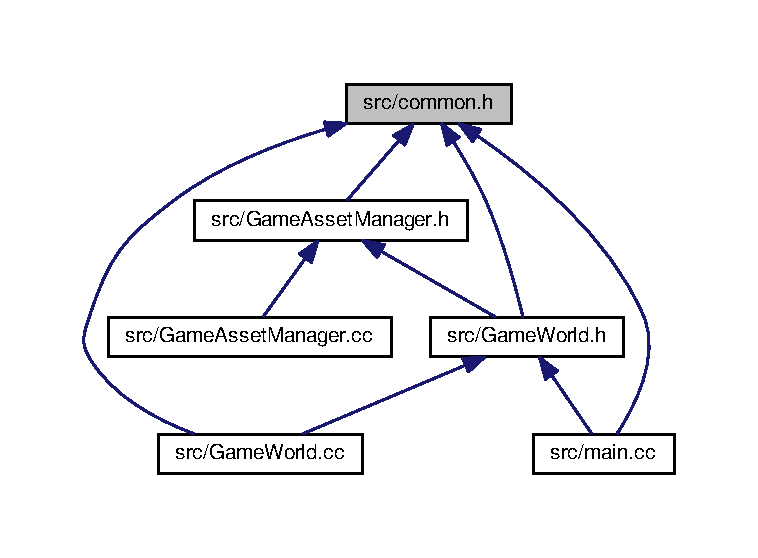
\includegraphics[width=350pt]{common_8h__dep__incl}
\end{center}
\end{figure}
\subsection*{Enumerations}
\begin{DoxyCompactItemize}
\item 
enum \hyperlink{common_8h_add86e7c88dd109abea3f708b422f31f0}{Application\+Mode} \{ \hyperlink{common_8h_add86e7c88dd109abea3f708b422f31f0a25f73324dc93d9024c0c75b4e6815335}{T\+R\+A\+N\+S\+F\+O\+R\+M}, 
\hyperlink{common_8h_add86e7c88dd109abea3f708b422f31f0a3dcfe0046eb5876e287dbf0914819b16}{R\+O\+T\+A\+T\+E}, 
\hyperlink{common_8h_add86e7c88dd109abea3f708b422f31f0a593be05a10070b4e7e0856e20590eaaf}{S\+C\+A\+L\+E}
 \}\begin{DoxyCompactList}\small\item\em Application\+Mode denotes the global state of the application. \end{DoxyCompactList}
\end{DoxyCompactItemize}


\subsection{Enumeration Type Documentation}
\hypertarget{common_8h_add86e7c88dd109abea3f708b422f31f0}{}\index{common.\+h@{common.\+h}!Application\+Mode@{Application\+Mode}}
\index{Application\+Mode@{Application\+Mode}!common.\+h@{common.\+h}}
\subsubsection[{Application\+Mode}]{\setlength{\rightskip}{0pt plus 5cm}enum {\bf Application\+Mode}}\label{common_8h_add86e7c88dd109abea3f708b422f31f0}


Application\+Mode denotes the global state of the application. 

There are three global states for this application\+:
\begin{DoxyEnumerate}
\item Transform -- load the correct shaders to do a transformation of a simple asset.
\item Rotate -- load the correct shader to rotate a simple asset.
\item Scale -- load the correct shader to scale a simple asset. 
\end{DoxyEnumerate}\begin{Desc}
\item[Enumerator]\par
\begin{description}
\index{T\+R\+A\+N\+S\+F\+O\+R\+M@{T\+R\+A\+N\+S\+F\+O\+R\+M}!common.\+h@{common.\+h}}\index{common.\+h@{common.\+h}!T\+R\+A\+N\+S\+F\+O\+R\+M@{T\+R\+A\+N\+S\+F\+O\+R\+M}}\item[{\em 
\hypertarget{common_8h_add86e7c88dd109abea3f708b422f31f0a25f73324dc93d9024c0c75b4e6815335}{}T\+R\+A\+N\+S\+F\+O\+R\+M\label{common_8h_add86e7c88dd109abea3f708b422f31f0a25f73324dc93d9024c0c75b4e6815335}
}]\index{R\+O\+T\+A\+T\+E@{R\+O\+T\+A\+T\+E}!common.\+h@{common.\+h}}\index{common.\+h@{common.\+h}!R\+O\+T\+A\+T\+E@{R\+O\+T\+A\+T\+E}}\item[{\em 
\hypertarget{common_8h_add86e7c88dd109abea3f708b422f31f0a3dcfe0046eb5876e287dbf0914819b16}{}R\+O\+T\+A\+T\+E\label{common_8h_add86e7c88dd109abea3f708b422f31f0a3dcfe0046eb5876e287dbf0914819b16}
}]\index{S\+C\+A\+L\+E@{S\+C\+A\+L\+E}!common.\+h@{common.\+h}}\index{common.\+h@{common.\+h}!S\+C\+A\+L\+E@{S\+C\+A\+L\+E}}\item[{\em 
\hypertarget{common_8h_add86e7c88dd109abea3f708b422f31f0a593be05a10070b4e7e0856e20590eaaf}{}S\+C\+A\+L\+E\label{common_8h_add86e7c88dd109abea3f708b422f31f0a593be05a10070b4e7e0856e20590eaaf}
}]\end{description}
\end{Desc}

\begin{DoxyCode}
12 \{\hyperlink{common_8h_add86e7c88dd109abea3f708b422f31f0a25f73324dc93d9024c0c75b4e6815335}{TRANSFORM}, \hyperlink{common_8h_add86e7c88dd109abea3f708b422f31f0a3dcfe0046eb5876e287dbf0914819b16}{ROTATE}, \hyperlink{common_8h_add86e7c88dd109abea3f708b422f31f0a593be05a10070b4e7e0856e20590eaaf}{SCALE}\};
\end{DoxyCode}

\hypertarget{CubeAsset_8cc}{}\section{src/\+Cube\+Asset.cc File Reference}
\label{CubeAsset_8cc}\index{src/\+Cube\+Asset.\+cc@{src/\+Cube\+Asset.\+cc}}
{\ttfamily \#include \char`\"{}Cube\+Asset.\+h\char`\"{}}\\*
Include dependency graph for Cube\+Asset.\+cc\+:
% FIG 0
\subsection*{Macros}
\begin{DoxyCompactItemize}
\item 
\#define \hyperlink{CubeAsset_8cc_a75f201b0e53e68726854997957322b8d}{check\+G\+L\+Error}()
\end{DoxyCompactItemize}


\subsection{Macro Definition Documentation}
\hypertarget{CubeAsset_8cc_a75f201b0e53e68726854997957322b8d}{}\index{Cube\+Asset.\+cc@{Cube\+Asset.\+cc}!check\+G\+L\+Error@{check\+G\+L\+Error}}
\index{check\+G\+L\+Error@{check\+G\+L\+Error}!Cube\+Asset.\+cc@{Cube\+Asset.\+cc}}
\subsubsection[{check\+G\+L\+Error}]{\setlength{\rightskip}{0pt plus 5cm}\#define check\+G\+L\+Error(
\begin{DoxyParamCaption}
{}
\end{DoxyParamCaption}
)}\label{CubeAsset_8cc_a75f201b0e53e68726854997957322b8d}

\hypertarget{CubeAsset_8h}{}\section{src/\+Cube\+Asset.h File Reference}
\label{CubeAsset_8h}\index{src/\+Cube\+Asset.\+h@{src/\+Cube\+Asset.\+h}}
{\ttfamily \#include $<$vector$>$}\\*
{\ttfamily \#include $<$G\+L/gl.\+h$>$}\\*
{\ttfamily \#include $<$glm/glm.\+hpp$>$}\\*
{\ttfamily \#include $<$glm/ext.\+hpp$>$}\\*
{\ttfamily \#include \char`\"{}Game\+Asset.\+h\char`\"{}}\\*
Include dependency graph for Cube\+Asset.\+h\+:
% FIG 0
This graph shows which files directly or indirectly include this file\+:
% FIG 1
\subsection*{Classes}
\begin{DoxyCompactItemize}
\item 
class \hyperlink{classCubeAsset}{Cube\+Asset}
\end{DoxyCompactItemize}

\hypertarget{GameAsset_8h}{}\section{src/\+Game\+Asset.h File Reference}
\label{GameAsset_8h}\index{src/\+Game\+Asset.\+h@{src/\+Game\+Asset.\+h}}
{\ttfamily \#include $<$iostream$>$}\\*
{\ttfamily \#include $<$G\+L/gl.\+h$>$}\\*
Include dependency graph for Game\+Asset.\+h\+:
% FIG 0
This graph shows which files directly or indirectly include this file\+:
% FIG 1
\subsection*{Classes}
\begin{DoxyCompactItemize}
\item 
class \hyperlink{classGameAsset}{Game\+Asset}
\end{DoxyCompactItemize}

\hypertarget{GameAssetManager_8cc}{}\section{src/\+Game\+Asset\+Manager.cc File Reference}
\label{GameAssetManager_8cc}\index{src/\+Game\+Asset\+Manager.\+cc@{src/\+Game\+Asset\+Manager.\+cc}}
{\ttfamily \#include \char`\"{}Game\+Asset\+Manager.\+h\char`\"{}}\\*
Include dependency graph for Game\+Asset\+Manager.\+cc\+:
% FIG 0

\hypertarget{GameAssetManager_8h}{}\section{src/\+Game\+Asset\+Manager.h File Reference}
\label{GameAssetManager_8h}\index{src/\+Game\+Asset\+Manager.\+h@{src/\+Game\+Asset\+Manager.\+h}}
{\ttfamily \#include $<$memory$>$}\\*
{\ttfamily \#include $<$vector$>$}\\*
{\ttfamily \#include $<$string$>$}\\*
{\ttfamily \#include $<$utility$>$}\\*
{\ttfamily \#include $<$fstream$>$}\\*
{\ttfamily \#include $<$iostream$>$}\\*
{\ttfamily \#include $<$G\+L/gl.\+h$>$}\\*
{\ttfamily \#include \char`\"{}common.\+h\char`\"{}}\\*
{\ttfamily \#include \char`\"{}Game\+Asset.\+h\char`\"{}}\\*
Include dependency graph for Game\+Asset\+Manager.\+h\+:
\nopagebreak
\begin{figure}[H]
\begin{center}
\leavevmode
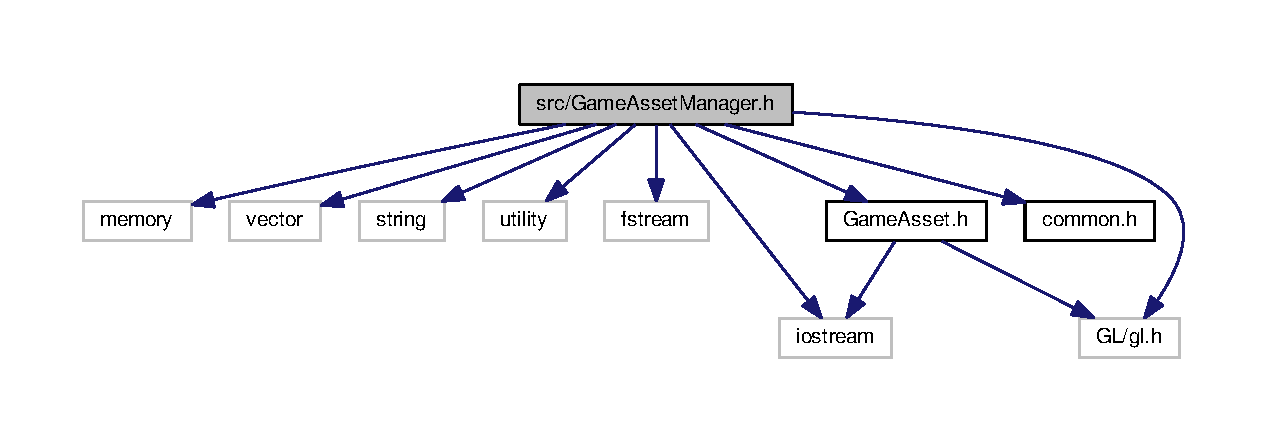
\includegraphics[width=350pt]{GameAssetManager_8h__incl}
\end{center}
\end{figure}
This graph shows which files directly or indirectly include this file\+:
\nopagebreak
\begin{figure}[H]
\begin{center}
\leavevmode
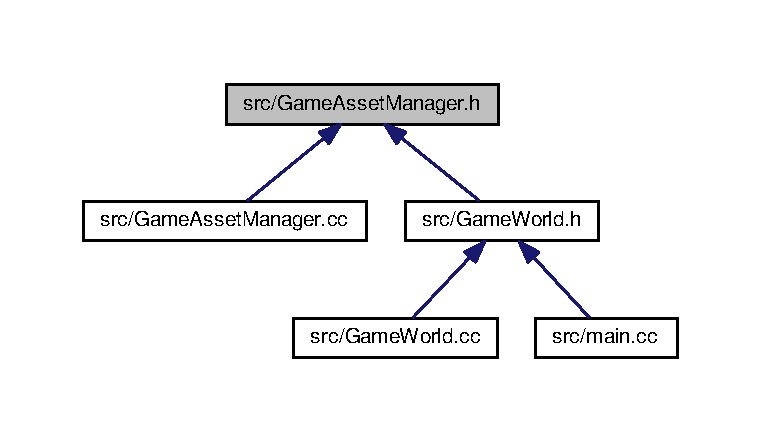
\includegraphics[width=350pt]{GameAssetManager_8h__dep__incl}
\end{center}
\end{figure}
\subsection*{Classes}
\begin{DoxyCompactItemize}
\item 
class \hyperlink{classGameAssetManager}{Game\+Asset\+Manager}
\begin{DoxyCompactList}\small\item\em \hyperlink{classGameAssetManager}{Game\+Asset\+Manager} is a container for Game\+Assets. \end{DoxyCompactList}\end{DoxyCompactItemize}

\hypertarget{GameWorld_8cc}{}\section{src/\+Game\+World.cc File Reference}
\label{GameWorld_8cc}\index{src/\+Game\+World.\+cc@{src/\+Game\+World.\+cc}}
{\ttfamily \#include \char`\"{}Game\+World.\+h\char`\"{}}\\*
{\ttfamily \#include \char`\"{}common.\+h\char`\"{}}\\*
Include dependency graph for Game\+World.\+cc\+:
\nopagebreak
\begin{figure}[H]
\begin{center}
\leavevmode
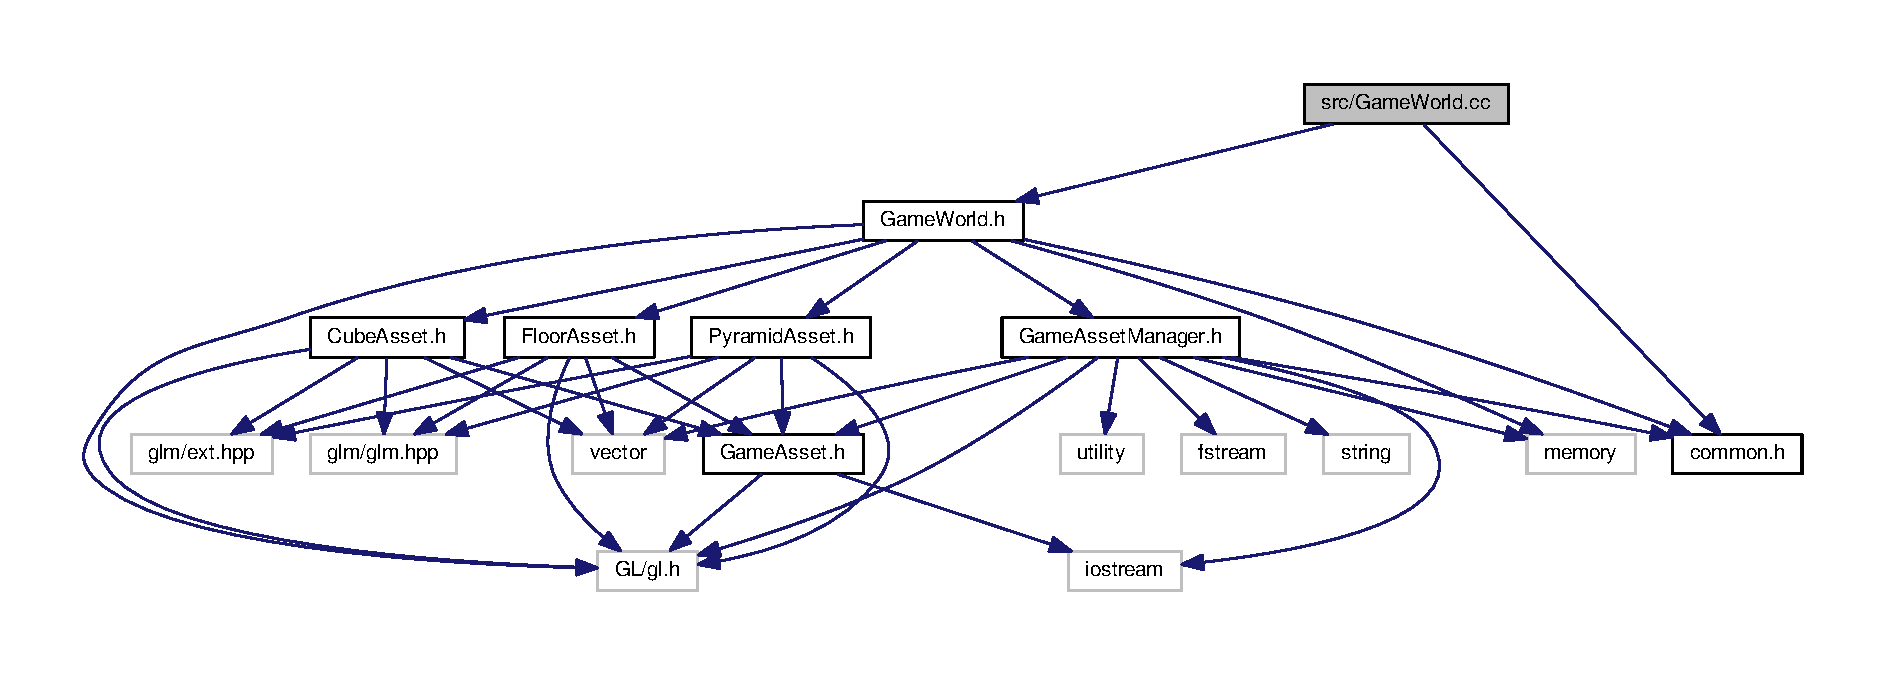
\includegraphics[width=350pt]{GameWorld_8cc__incl}
\end{center}
\end{figure}

\hypertarget{GameWorld_8h}{}\section{src/\+Game\+World.h File Reference}
\label{GameWorld_8h}\index{src/\+Game\+World.\+h@{src/\+Game\+World.\+h}}
{\ttfamily \#include $<$memory$>$}\\*
{\ttfamily \#include $<$G\+L/gl.\+h$>$}\\*
{\ttfamily \#include \char`\"{}common.\+h\char`\"{}}\\*
{\ttfamily \#include \char`\"{}Game\+Asset\+Manager.\+h\char`\"{}}\\*
{\ttfamily \#include \char`\"{}Cube\+Asset.\+h\char`\"{}}\\*
{\ttfamily \#include \char`\"{}Pyramid\+Asset.\+h\char`\"{}}\\*
Include dependency graph for Game\+World.\+h\+:
% FIG 0
This graph shows which files directly or indirectly include this file\+:
% FIG 1
\subsection*{Classes}
\begin{DoxyCompactItemize}
\item 
class \hyperlink{classGameWorld}{Game\+World}
\begin{DoxyCompactList}\small\item\em \hyperlink{classGameWorld}{Game\+World} allows us to separate the management of the game world from the nuts and bolts of game loop initialisation. \end{DoxyCompactList}\end{DoxyCompactItemize}

\hypertarget{main_8cc}{}\section{src/main.cc File Reference}
\label{main_8cc}\index{src/main.\+cc@{src/main.\+cc}}
{\ttfamily \#include \char`\"{}Game.\+h\char`\"{}}\\*
Include dependency graph for main.\+cc\+:
\nopagebreak
\begin{figure}[H]
\begin{center}
\leavevmode
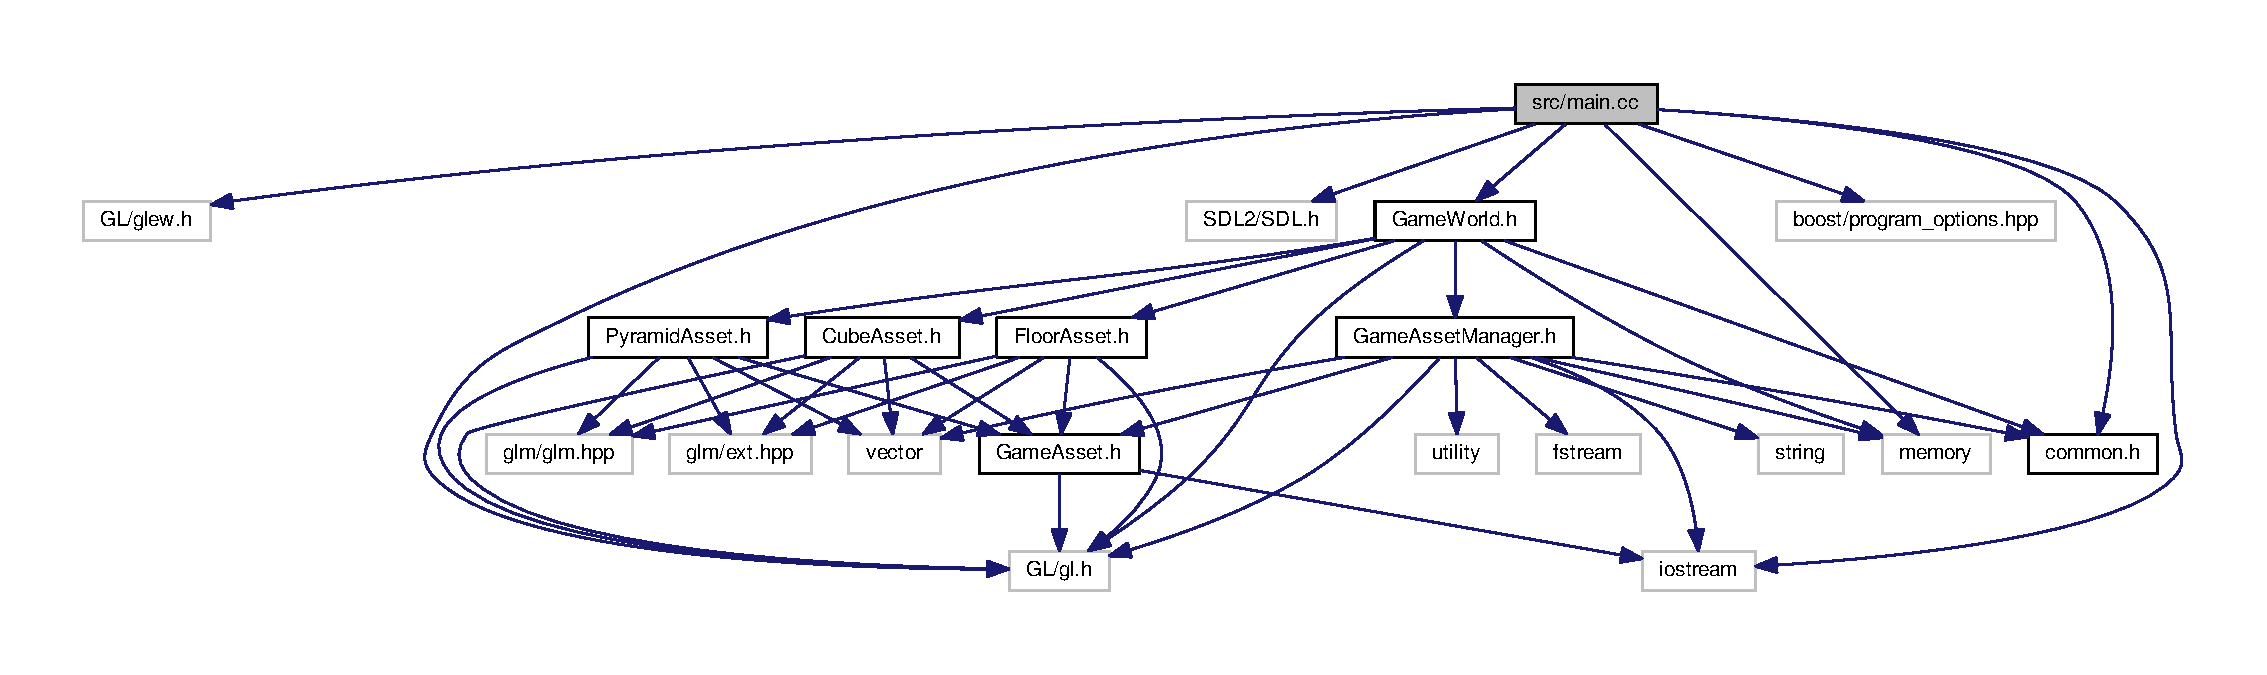
\includegraphics[width=350pt]{main_8cc__incl}
\end{center}
\end{figure}
\subsection*{Functions}
\begin{DoxyCompactItemize}
\item 
int \hyperlink{main_8cc_ae66f6b31b5ad750f1fe042a706a4e3d4}{main} ()
\end{DoxyCompactItemize}


\subsection{Function Documentation}
\hypertarget{main_8cc_ae66f6b31b5ad750f1fe042a706a4e3d4}{}\index{main.\+cc@{main.\+cc}!main@{main}}
\index{main@{main}!main.\+cc@{main.\+cc}}
\subsubsection[{main()}]{\setlength{\rightskip}{0pt plus 5cm}int main (
\begin{DoxyParamCaption}
{}
\end{DoxyParamCaption}
)}\label{main_8cc_ae66f6b31b5ad750f1fe042a706a4e3d4}
Main Runs the \hyperlink{class_game}{Game} file which handles the main loop of the game. 
\hypertarget{PyramidAsset_8cc}{}\section{src/\+Pyramid\+Asset.cc File Reference}
\label{PyramidAsset_8cc}\index{src/\+Pyramid\+Asset.\+cc@{src/\+Pyramid\+Asset.\+cc}}
{\ttfamily \#include \char`\"{}Pyramid\+Asset.\+h\char`\"{}}\\*
Include dependency graph for Pyramid\+Asset.\+cc\+:
\nopagebreak
\begin{figure}[H]
\begin{center}
\leavevmode
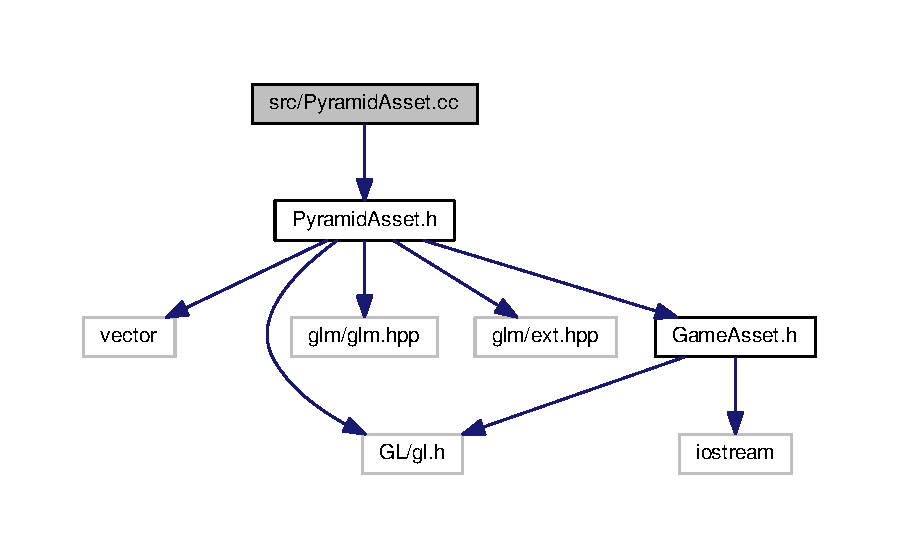
\includegraphics[width=350pt]{PyramidAsset_8cc__incl}
\end{center}
\end{figure}
\subsection*{Macros}
\begin{DoxyCompactItemize}
\item 
\#define \hyperlink{PyramidAsset_8cc_a75f201b0e53e68726854997957322b8d}{check\+G\+L\+Error}()
\end{DoxyCompactItemize}


\subsection{Macro Definition Documentation}
\hypertarget{PyramidAsset_8cc_a75f201b0e53e68726854997957322b8d}{}\index{Pyramid\+Asset.\+cc@{Pyramid\+Asset.\+cc}!check\+G\+L\+Error@{check\+G\+L\+Error}}
\index{check\+G\+L\+Error@{check\+G\+L\+Error}!Pyramid\+Asset.\+cc@{Pyramid\+Asset.\+cc}}
\subsubsection[{check\+G\+L\+Error}]{\setlength{\rightskip}{0pt plus 5cm}\#define check\+G\+L\+Error(
\begin{DoxyParamCaption}
{}
\end{DoxyParamCaption}
)}\label{PyramidAsset_8cc_a75f201b0e53e68726854997957322b8d}

\hypertarget{PyramidAsset_8h}{}\section{src/\+Pyramid\+Asset.h File Reference}
\label{PyramidAsset_8h}\index{src/\+Pyramid\+Asset.\+h@{src/\+Pyramid\+Asset.\+h}}
{\ttfamily \#include $<$vector$>$}\\*
{\ttfamily \#include $<$G\+L/gl.\+h$>$}\\*
{\ttfamily \#include $<$glm/glm.\+hpp$>$}\\*
{\ttfamily \#include $<$glm/ext.\+hpp$>$}\\*
{\ttfamily \#include \char`\"{}Game\+Asset.\+h\char`\"{}}\\*
Include dependency graph for Pyramid\+Asset.\+h\+:
\nopagebreak
\begin{figure}[H]
\begin{center}
\leavevmode
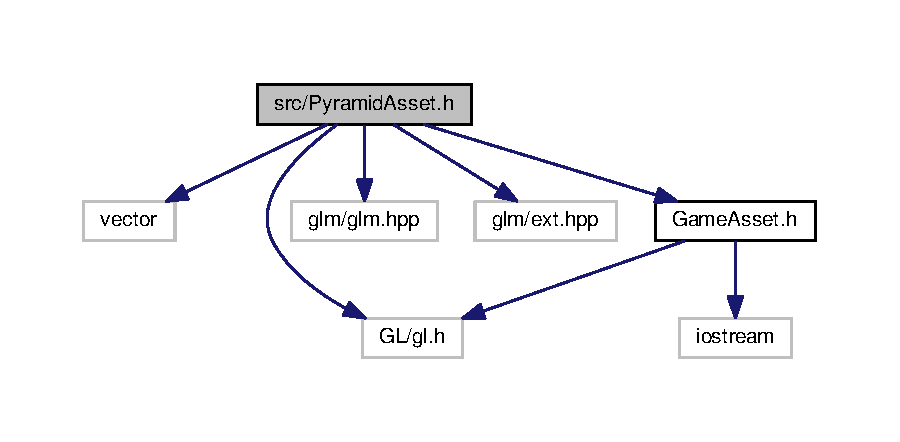
\includegraphics[width=350pt]{PyramidAsset_8h__incl}
\end{center}
\end{figure}
This graph shows which files directly or indirectly include this file\+:
\nopagebreak
\begin{figure}[H]
\begin{center}
\leavevmode
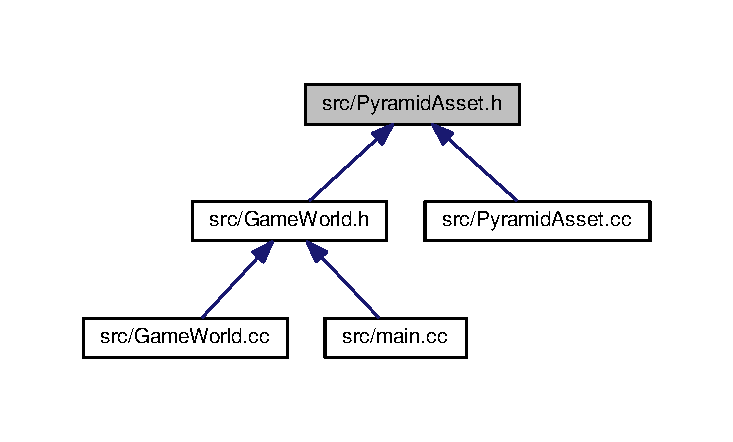
\includegraphics[width=350pt]{PyramidAsset_8h__dep__incl}
\end{center}
\end{figure}
\subsection*{Classes}
\begin{DoxyCompactItemize}
\item 
class \hyperlink{classPyramidAsset}{Pyramid\+Asset}
\end{DoxyCompactItemize}

%--- End generated contents ---

% Index
\backmatter
\newpage
\phantomsection
\clearemptydoublepage
\addcontentsline{toc}{chapter}{Index}
\printindex

\end{document}
